
\provideboolean{Slides}
\setboolean{Slides}{false}

\begin{frontmatter}%

  \chapter[Chapter Title]{Epidemiological Expectations in Economics\footnote{We would like to thank xxx, xxx for comments.}}\label{chap1}

  % \subtitle{Chapter Subtitle}

  \author*[1]{Christopher Carroll}%
  \author[2]{Tao Wang}%

  \address[1]{\orgname{Johns Hopkins University}, \orgdiv{Department of Economics}, \orgaddress{Baltimore, Maryland}}
  \address[2]{\orgname{Johns Hopkins University}, \orgdiv{Department of Economics}, \orgaddress{Baltimore, Maryland}}
  \address*[3]{Corresponding: \email{twang80@jhu.edu}}

  
  % \authormark{First Author, Second Author and Third Author}
  \titlemark{Part Title}
  \chaptermark{Epidemiological Expectations in Economics}

  \MaxmMiniTocnum{A.1}{3.3.3}{}

  \minitoc

  \makechaptertitle

  \begin{abstract}[Abstract]
    `Epidemiological' models of belief dynamics put social interactions at their core; such models are the main (almost, the only) tool used by non-economists to study how beliefs evolve in populations.  We survey the (comparatively) small literature in which economists attempting to model the consequences of beliefs about the future -- `expectations' -- have employed a full-fledged epidemiological approach to explore an economic question.  We draw connections to related work on narrative economics, news/rumor spreading, `contagion,' and the spread of online content. Finally, we discuss a number of promising directions for future research.
  \end{abstract}

  \begin{keywords}[Keywords:]
    Economic Expectations \sep Epidemiological Expectations \sep Social interactions \sep Social dynamics \sep Information diffusion \sep Economic Narratives
  \end{keywords}

\begin{verbatimwrite}{./Slides/QuoteArrow1969}%%%Slides
  \begin{quote}
    While mass media play a major role in alerting individuals to the
    possibility of an innovation, it seems to be personal contact that is
    most relevant in leading to its adoption. Thus, the diffusion of an
    innovation becomes a process formally akin to the spread of an
    infectious disease.
    \source{\href{https://github.com/iworld1991/EpiExp/blob/master/Literature/arrow_classificatory_1969.pdf}{\cite{arrow_classificatory_1969}}}
  \end{quote}
\end{verbatimwrite} %%%Slides
%%%Slides
  \begin{quote}
    While mass media play a major role in alerting individuals to the
    possibility of an innovation, it seems to be personal contact that is
    most relevant in leading to its adoption. Thus, the diffusion of an
    innovation becomes a process formally akin to the spread of an
    infectious disease.
    \source{\href{https://github.com/iworld1991/EpiExp/blob/master/Literature/arrow_classificatory_1969.pdf}{\cite{arrow_classificatory_1969}}}
  \end{quote}
 %%%Slides

\begin{verbatimwrite}{./Slides/QuoteSimon1984}%%%Slides
\begin{quote}\ifthenelse{\boolean{Slides}}{\footnotesize}{}
	A very natural next step for economics is to maintain expectations in
	the strategic position they have come to occupy, but to build an
	empirically validated theory of how attention is in fact directed within
	a social system, and how expectations are, in fact, formed.
	\source{\href{https://econpapers.repec.org/RePEc:eee:jeborg:v:5:y:1984:i:1:p:35-55}{\cite{simon_behavioral_1984}}}
\end{quote}
\end{verbatimwrite} %%%Slides
%%%Slides
\begin{quote}\ifthenelse{\boolean{Slides}}{\footnotesize}{}
	A very natural next step for economics is to maintain expectations in
	the strategic position they have come to occupy, but to build an
	empirically validated theory of how attention is in fact directed within
	a social system, and how expectations are, in fact, formed.
	\source{\href{https://econpapers.repec.org/RePEc:eee:jeborg:v:5:y:1984:i:1:p:35-55}{\cite{simon_behavioral_1984}}}
\end{quote}
 %%%Slides

\begin{verbatimwrite}{./Slides/QuoteShiller2017}%%%Slides
  \begin{quote}
    If we want to know why an unusually large economic event happened, we
    need to list the seemingly unrelated narratives that all happened to be
    going viral at around the same time and affecting the economy in the
    same direction.
    \source{\href{https://www.amazon.in/Narrative-Economics-Stories-Economic-Events-ebook/dp/B07RRDVTHY}{\cite{shiller2017narrative}}}
  \end{quote}
\end{verbatimwrite} %%%Slides
%%%Slides
  \begin{quote}
    If we want to know why an unusually large economic event happened, we
    need to list the seemingly unrelated narratives that all happened to be
    going viral at around the same time and affecting the economy in the
    same direction.
    \source{\href{https://www.amazon.in/Narrative-Economics-Stories-Economic-Events-ebook/dp/B07RRDVTHY}{\cite{shiller2017narrative}}}
  \end{quote}
 %%%Slides

\begin{verbatimwrite}{./Slides/QuoteInception2010}%%%Slides
\begin{quote}
An idea is like a virus. Resilient. Highly contagious. And even the smallest seed of an idea can grow.   --Cobb

  \source{The movie Inception (2010)} % Tao: Fix citation
\end{quote}
\end{verbatimwrite} %%%Slides
%%%Slides
\begin{quote}
An idea is like a virus. Resilient. Highly contagious. And even the smallest seed of an idea can grow.   --Cobb

  \source{The movie Inception (2010)} % Tao: Fix citation
\end{quote}
 %%%Slides

  % \begin{points}[Chapter Points]
  %   \begin{itemize}
  %   \item{} The result of this approach is to produce a top-down view of it is a framework
  %     that standardizes the manner in which organizations.
  %   \item{} Complex data content, thereby reducing the overheads associated with acquiring,
  %     organizing and managing data content.  Using such a framework in turn supports an incremental approach
  %     to improving business applications.
  %   \item{} Standardizes the manner in which organizations.
  %   \end{itemize}%
  % \end{points}%

\end{frontmatter}%

\section{Introduction}
\label{chap1:sec1}

It is a commonplace, in academia and popular culture, that ideas spread like diseases: they can be ``infectious'' or ``go viral.''  The proposition is hardly new; as \cite{shiller2017narrative} points out, it can be found at least as far back as \cite{humeenquiry},
 whose ideas thoroughly infected the work of his friend \cite{smithwealth}.\footnote{See \cite{rasmussen2017infidel}.} Indeed, %with one notable exception (see below),
 debates in fields other than economics are rarely about whether social interactions are fundamental; the debate is about which particular models for capturing social interactions are most suitable for understanding the spread of which kinds of ideas.

``Expectations'' are just a category of ideas.  So upon being told that expectations play a critical role in structural economic modeling, a scholar who was not an economist might suppose that epidemiological models of  expectations would be a standard part of the economist's modeling toolkit --- unless there were good reason to suppose that economic ideas are immune to social influence.

But evidence for social transmission of economic ideas is plentiful and has recently been growing by leaps and bounds -- see Section~\ref{subsec:microEvidence} for a sampling.  Still, it would not be accurate to say that an `epidemiological expectations' (`EE') approach is a standard way of constructing formal models of economic phenomena -- as a conventional off-the-shelf alternative, say, to a `rational expectations' (`RE') approach, the `Rational Inattention' (`RI') approach advocated by~\cite{sims2003implications}, or even to the `diagnostic expectations' model of~\cite{bordalo2018diagnostic}, or a number of bounded rationality approaches (e.g.,~\cite{gabaix2020behavioral}).

Undoubtedly, one reason for this is that nowhere has any attempt been made to define what would constitute a full-fledged EE approach.

Despite this handicap, there have been some notable examples of what what we would describe as full-fledged EE models, which we define as requiring the following elements (in addition to whatever might be included in a model in which expectations are determined in some other way):
\begin{verbatimwrite}{./Slides/FullFledgedEE}
\begin{quote}\normalfont
\begin{enumerate}
\item mechanism: \ifthenelse{\boolean{Slides}}{math by which idea(s) transmitted}{An explicit and rigorous mathematical description of an interaction in which idea(s) are transmitted among agents  ...}
\item dynamics: \ifthenelse{\boolean{Slides}}{
    ... that $\mathbb{E}$ dynamics (micro and popn) ...
}
{... that (at least in principle) generates observable expectation dynamics...}
\item economic: \ifthenelse{\boolean{Slides}}{... those $\mathbb{E} \Rightarrow$ an economic outcome}{
... and those expectations have knock-on consequences for an observable outcome (often, prices, quantities, or market values) that is a primary subject of the economic analysis}
  \end{enumerate}
\end{quote}
\end{verbatimwrite}
\begin{quote}\normalfont
\begin{enumerate}
\item mechanism: \ifthenelse{\boolean{Slides}}{math by which idea(s) transmitted}{An explicit and rigorous mathematical description of an interaction in which idea(s) are transmitted among agents  ...}
\item dynamics: \ifthenelse{\boolean{Slides}}{
    ... that $\mathbb{E}$ dynamics (micro and popn) ...
}
{... that (at least in principle) generates observable expectation dynamics...}
\item economic: \ifthenelse{\boolean{Slides}}{... those $\mathbb{E} \Rightarrow$ an economic outcome}{
... and those expectations have knock-on consequences for an observable outcome (often, prices, quantities, or market values) that is a primary subject of the economic analysis}
  \end{enumerate}
\end{quote}

  These criteria whittle down a vast number of invocations, or partial discussions, of the proposition that ideas spread through social interaction to the surprisingly small number of papers on which we primarily focus here.  (The last criterion allows us to neglect vast literatures on public opinion, politics, musical tastes, and other topics).

\section{Background and Motivation}\label{motivation-and-context}

% We begin with developments in connected areas that may be helpful in understanding the trajectory of epidemiological expectations modeling  in economics.

\subsection{Expectational Heterogeneity}\label{EpiExpHet}\hypertarget{EpiExpHet}{}
%\subsubsection{Expectations are Heterogeneous}\label{expectations-are-heterogeneous}\hypertarget{ExpectationsAreHeterogeneous}{}

\begin{verbatimwrite}{./Slides/QuoteBrowningHansenHeckman1999}%%%Slides
    In their introduction to the \textit{Handbook of Microeconomics}\href{http://larspeterhansen.org/wp-content/uploads/2016/11/Microdata-and-GE-Models.pdf}{Browning, Heckman, and Hansen \citeyear{browning_chapter_1999}}, wrote that the most universal lesson of micro economics is that ``people are different in ways that importantly affect their economic behavior.''
\end{verbatimwrite}%%%Slides
%%%Slides
    In their introduction to the \textit{Handbook of Microeconomics}\href{http://larspeterhansen.org/wp-content/uploads/2016/11/Microdata-and-GE-Models.pdf}{Browning, Heckman, and Hansen \citeyear{browning_chapter_1999}}, wrote that the most universal lesson of micro economics is that ``people are different in ways that importantly affect their economic behavior.''
%%%Slides
\begin{verbatimwrite}{./Slides/subsubsecExpAreHet}

\end{verbatimwrite}
    Over the subsequent two decades, a great deal of the progress in macro economics has come from incorporating microeconomic heterogeneity ``in ways that importantly affect'' macroeconomic behavior.  (See ``Macroeconomics and Heterogeneity'' in the 2020 \textit{Handbook of Macroeconomics} \cite{kmpHandbook}).  In particular, Heterogeneous Agent  (`HA-Macro') models that match the distributions of income and wealth
    have now provided rigorous microfoundations for Keynesian macroeconomics by capturing measured heterogeneity in (and a large average value for) the marginal propensity to consume -- see \cite{violante_marginal_2021}'s Laffont lecture.

%\subsubsection{Expectational Heterogeneity Is Rarely Modeled}\label{Expectational-heterogeneity-is-rarely-modeled}\hypertarget{expectational-heterogeneityIsRarelyModeled}
    But only a few structural models in the HA-Macro literature have allowed for differences in agents' expectations about variables like stock returns (where everyone's realized outcome will be identical) -- even though disagreements on such subjects are large and people make choices that correspond -- at least somewhat --  to their expressed beliefs (\cite{gmsuBeliefs}).

    Partly, the omission of expectational heterogeneity may reflect the fact that until recently there was not widespread awareness among macroeconomists that measurable microeconomic expectations have considerable power to explain observable microeconomic behavior -- see the published discussions in the 2017 NBER Macroeconomics Annual of~\cite{manski2017survey}'s paper surveying the literature on the measurement of expectations, in which Manski himself has been the leading figure (and until recently something of a lone voice crying in the wilderness).%, until the  recent change reflected upon in the favorable reception of his paper both by his discussants and by the conference attendees.

    Other signs of the new focus on the measurement of expectations are developments like the commissioning of this \emph{Handbook of Economic Expectations}, the creation of the \emph{Survey of Consumer Expectations} by the Federal Reserve Bank of New York in 2014 % Tao: citation
    (and several similar surveys in other places), and the fact that questions on expectations have begun to be added to existing surveys like the ones used for calibrating HA-Macro models.  %The HRS, for example, collects expectations about stock returns, and~\cite{mv77PortfolioNonPuzzle} shows both that HRS respondents are systematically pessimistic (relative to economists's views) and that the more pessimistic a respondent is, the less likely they are to invest.

    But EE modeling approaches may be particularly appealing now as a result of the emergence of new \emph{kinds} of data.  In particular, for the first time ever, it is now becoming possible to directly observe economic expectations spreading over social networks -- as is done in the paper we describe below by~\cite{bailey2018economic}.

\subsection{Epistemology and Epidemiology}

    One aspect of the EE approach that seems to trouble economists more than scholars from other fields is the requirement to specify a source for the idea(s) whose spread is being modeled.

    The Rational Expectations approach gets around this problem (even in the HA-Macro world) by making some rather bold assumptions (there is only one `true' model of the world; everyone believes the same true model; everyone observes all relevant facts and draws the same conclusions from them; and so on).  %The reward for this steep price is that often RE models have a unique and testable equilibrium.

    Such models are often not easy to understand, and is not unreasonable to worry that the added complexity from an epidemiological mechanism of belief transmission will add more confusion than explanation.

    One solution is for economists to study models with agents whose expectations formation mechanism is `tunable' in the degree to which it differs from better-understood models (RE or not).  This should not be too hard:  If the only `source' of ideas is an agent who believes in the rational expectations solution, and the infection rate is 100 percent, the solution will be the rational expectations solution.  More interesting epidemiological mechanisms can build from there.

    In fact, most of the examples of EE models we highlight are of this kind: There is some parameter or set of parameters can be set to zero (or infinity, or some other specific value), causing the model to collapse to an off-the-shelf rational expectations model.  See section~\ref{subsec:macroExp} for discussion of some specific examples.

\begin{comment}
    The literature's many informal references to epidemiological ideas indicate  that economists are familiar with these ideas and find them tempting.  The hesitancy to adopt explicitly epidemiological methods in the analysis of standard economic questions therefore seems unlikely to reflect a consensus that there are no plausible epidemiological models; it seems more  likely to reflect a concern that there are too many.  Without considerable further discipline beyond the proposition that `ideas spread like diseases' it is not unreasonable to worry about whether an `epidemiological expectations' approach is sufficiently well defined to be worth exploring.
%\subsubsection{Why Identical Rational Expectations Remain the Default}\label{subsubsec:expectations-are-heterogeneous}\hypertarget{WhyIdentical RationalExpectationsRemainTheDefault}{}
     ``Rational Expectations'' (`RE') -- which in this context really means `identical expectations' --  remains a default at least partly because it usually can generate unique and testable predictions for the dynamics of aggregate variables.

    But several counterpoints are worth emphasizing.

    The first is that expectations are \textit{measurable}, and increasingly measured in the kinds of micro datasets used to calibrate and simulate HA-macro models.  All survey data (including income and wealth) need to be treated carefully to guard against measurement problems, and the extensive literature on the measurement of expectations suggests that those data should be treated with particular care -- but also demonstrates that robust information is contained in the answers to such questions.

    Thus, EE models have a source of discipline unavailable in the RE framework. This fact could help counter concerns about whether such models provide too many degrees of freedom to be usefully testable.


    % -- even if solving RA models in the presence of nonexpectational heterogeneity (wealth; income) is a major challenge.  %But the HA-Macro literature has helped macroeconomists get comfortable with results that emerge from the simulation of large populations of agents all of whom are in different circumstances.

\begin{comment}
    RE also corresponds rather directly to philosophers' traditional formulation of how humans can come to know things: A solitary reasoner has some fundamental assumptions about the world and makes logical/mathematical deductions to construct beliefs about things not directly observable (like, the future).\footnote{See Bertrand~\citep{russell1946history} for a history that traces these ideas all the way back to Plato and Aristotle.}%\footnote{\cite{broad1952ethics} is a descendant of Hume's: \href{https://en.wikipedia.org/wiki/Problem_of_induction}{``Induction is the glory of science and the scandal of philosophy''.}}

    Yet even in philosophy there is a growing recognition that most knowledge that people (think they) possess cannot possibly be so hard-core.  As \cite{coady1992testimony}, an early advocate of ``social epistemology,'' puts it, many of us have never directly observed the delivery of a baby, yet we have firm convictions about how it happens.  And most of us have not mastered the skills necessary to prove by personal observation of sunrises and sunsets (and intricate mathematical deduction) that the Earth is (roughly) spherical.  We believe that the Earth is spherical, and a great many other things, because to a large degree we trust the testimony of other people who tell us that they have collected the facts and done the math.

    %In some cases, the RE equilibrium is the eventual limit of a process of social interaction (a model of scientific belief transmission may imply that there are fewer members of the Flat Earth Society with each passing year).  But even in those epidemiological models where convergence occurs, a difference with the RE model is that the process of reaching consensus takes time rather than being instantaneous.

    % Keynes quotes:

    % "If we speak frankly, we have to admit that our basis of knowledge for estimating the yield ten years hence of a railway, a copper mine, a textile factory, the goodwill of a patent medicine, an Atlantic liner, a building in the City of London amounts to little and sometimes to nothing"

    % "Even apart from the instability due to speculation, there is the instability due to the characteristic of human nature that a large proportion of our positive activities depend on spontaneous optimism her thanher than on a mathematical expectation, whether moral or hedonistic or economic. Most, probably, of our decisions to do something positive, the full consequences of which will be drawn out over many days to come, can only be taken as a result of animal spiritsof a spontaneous urge to action rather than inaction, and not as the outcome of a weighted average of quantitative benefits multiplied by"

    % The sensible question, then, is how best to model the ways in which external sources of information produce individuals' beliefs. %This is the potential point of entry for epidemiological models:  As a mathematical or computational matter, there is little difference in the set of ways in which information might be transmitted from person to person (or common source to person) and the ways in which infection might be transmitted.
\end{comment}

\subsection{Epidemiology on Networks}
%\subsubsection{Consequences of Social Transmission}\label{subsubsec:Consequences-of-Social-Transmission}\hypertarget{ConsequencesOfSocialTransmission}{}

    For short, we use the word `classical' to refer to epidemiological models that descend from the work of \cite{kermack_contribution_1927}, who formulated the problem as one of tracking the size of `compartments' of the population in different disease states (like susceptible or infected) under a `random mixing' assumption in which all members of the population were equally likely to encounter each other in a time interval.  The random mixing assumption, along with the use of continuous time and real numbers for the compartment sizes, allowed the problem to be described by a set of differential equations which could be solved numerically even in 1927.

    A more recent literature also examines the social transmission of beliefs and satisfies any reasonable interpretation of  an `epidemiological' approach:  A large body of work using the tools of `network theory' studies models in which the `nodes' in a graph are interpreted as people and the `edges' are social connections between nodes, and the analysis aims to determine the consequences of modeling assumptions for the structure and flow of information (or beliefs, or ideas) in a finite population of agents over discrete time steps.\footnote{The mathematical formulation of network theory, or graph theory (the boundary between these is porous) is usually attributed to Leonhard Euler, in his solution to a problem of geography -- the ``Bridges of Konigsberg.''}  A standard reference for economists is the textbook by~\cite{jackson_social_2010}.

    While the two approaches seem quite different, it turns out that the network theory tools can be configured in such a way as to produce an arbitrarily close approximation to the solution to the original classical problem.  But they can also study a great many other essentially epidemiological questions that could not even be formulated in the classical setup.  (Network theory has also been used to study a wide range of questions in game theory and other fields quite distant from epidemiology.)

    %\subsubsection{Its A Small World After All}\label{subsubsec:Its-A-Small-World-After-All}\hypertarget{ItsASmallWorldAfterAll}{}

    One well-known network theory result that (to some extent) helps bridge the two approaches is the ``Small World'' effect first explained by~\cite{wsSmallWorld}, who articulate conditions under which even a small number of social connections can define a network in which virtually everyone is connected to everyone else by a small number of links.  \cite{barabasi2016network}'s summary is that when network models are calibrated to match measurable facts about human connections (or, for that matter, internet links), the ``interconnectedness'' phenomenon is extremely robust (which they point out holds across many competing models).

    This provides a satisfying explanation for a phenomenon first documented by \cite{milgram1967small}, who famously found that, on average, any two randomly selected people in the U.S.\ population were able to identify intermediate links of personal friends and friends-of-friends (and so on) by which they were connected, with the typical length of the chain involving only six people.\footnote{This is another example of crossover appeal in popular culture, having spawned John \cite{guareSixDegrees}'s play \href{https://en.wikipedia.org/wiki/Six_Degrees_of_Separation_(play)}{`Six Degrees of Separation'} a  \href{https://en.wikipedia.org/wiki/Six_Degrees_of_Separation_(film)}{movie} adaptation, a popular \href{https://en.wikipedia.org/wiki/Six_Degrees_of_Kevin_Bacon}{parlor game}, and other byproducts like calculators for the degrees of separation between \href{https://oakland.edu/enp/}{academics}).}  For our purposes, the interesting insight is that the ``Small Worlds'' phenomenon may suggest that the `random mixing' assumption typically made (and frequently objected to) in `classical' epidemiological models may not be as problematic as it might seem at first.

    % Although it is not usually motivated that way, a useful alternative foundation for the `identical foundations' approach can easily be constructed in a world where people trust external sources.

    %A vast literature outside of economics has investigated questions of this kind, as applied to topics like the diffusion of scientific knowledge~\cite{bettencourt2006power} or religious beliefs (\cite{hayward2018mathematical}).

    %The key point is best understood as follows.

    %A large literature in mathematics, beginning with \cite{erdos1960evolution}, has developed the pure theory, and more recently computational tools have allowed numerical investigations, but a fair distillation of much of this work would be to say

    % In this light, the fact that there are a few remaining members of the Flat Earth Society could be interpreted as evidence in favor of the philosopher-economist's point of view; those might be the unlucky people who made a math mistake which implied a pancake-shaped Earth, which could maybe be described as ``flat.''  Their imperviousness to the testimony of others could be interpreted as exemplifying people's ability to reach their own conclusions without regard to the common opinion of the crowd.

    % But the fact that almost everyone is ``connected'' in this sense is hardly sufficient to justify a conclusion that everyone has identical beliefs about everything.  That would require very strong auxiliary assumptions about the nature of communications across links.

    A distinct advantage of the `network' approach over the classical epidemiological approach is the extent to which, especially with modern computational tools, a network modeler can examine the consequences of almost arbitrarily rich assumptions about the exact nature of interactions between agents.  A key theme of the network literature is that even in a fully connected world, it is easy to construct models in which disagreement persists indefinitely (\cite{acemouglu2013opinion}) and subpopulations converge to different beliefs~\cite{sikder2020minimalistic}.  (The `clustering coefficient' which captures the extent to which your friends know each other is often -- though not always -- important in such models).

    % that would follow only under a host of additional assumptions which have widely varying plausibility for different kinds of knowledge or information transmission.  As a result, our survey will highlight models that deviate in interesting ways from the framework specified above.

\subsection{Expectational Tribes}\label{subsec:ExpTribes}

    We conclude the motivation by presenting some evidence that seems particularly compelling because it illustrates a recent clear failure of `identical beliefs' with consequences for choices in an area that is core to both micro and macro modeling: financial risk-taking.

    \href{https://github.com/iworld1991/EpiExp/blob/master/Literature/meeuwis2018belief.pdf}{\cite{meeuwis2018belief}}, using a dateset on millions of retirement investors from a large financial institution, show that after Donald Trump's surprise victory in the U.S.\ 2016 Presidential election, investors likely to be affiliated with Republican Party (inferred from  campaign donations at the zip code level) increased the equity share in their portfolio, while (likely) Democrats rebalanced into safe assets. These choices occurred at exactly the same time that consumer sentiment surveys showed that self-identified Republicans had suddenly become more optimistic, and Democrats more pessimistic, about the economy's prospects over the next few years.  The paper's rich dataset allows the authors to persuasively rule out non-belief-based channels (like income hedging needs, preferences, or local economic exposure). %Moreover, such differences in investment behaviors are found for investors working at the same employer and living in the same county.

%    After we articulate alternative epidemiological models of the spread of ideas, we will be in a position to discuss how evidence of this kind can be useful in winnowing the field of models.

\centerline{    [Insert Figure \ref{fig:parker} here]}

%    Some remaining assumptions that could justify an `identical expectations' equilibrium would be (1) there is a single, unambiguous truth about the state of the world; (2) all agents who make an observation about the world would perceive the same truth; (3) all agents truthfully communicate all their observations to all their links instantaneously; (4) everyone agrees about the correct model of how the world works.'

%    These assumptions effectively resurrect the identical expectations equilibrium in a framework where social communications exist, but achieve instantaneous and complete homogeneity in beliefs.  We can think of all of the epidemiological/network models discussed below as deviations, in one respect or another, from this perfect-trust instantaneous-transmission perfect-agreement framework.


\section{What insights can the epidemiological framework
  offer?}\label{what-insights-can-the-epidemiological-framework-offer}

\subsection{What Is an Epidemiological Framework?}
\label{subsec:epi_framework}

We will say that ideas, beliefs, `narratives,' or other mental states that can affect behavior
(henceforth, `expectations' will be shorthand for all of these) are the result of an ``epidemiological'' process whenever they are modeled as resulting from some social interaction.

This is a slightly narrower scope than the mechanisms encompassed in textbook
definitions of epidemiology, which can include the study of diseases that develop without any identifiable external influence.  The category of epidemiological models we are interested in is those for ``transmissible'' diseases.

But the transmission need not be person-to-person.   ``Common source''  diseases do not involve any one-on-one contact; for example, cosmic radiation to which everyone is exposed can cause diseases like cancer.  People living in caves would be less susceptible; those on mountaintops, more.

In the context of expectation formation a natural interpretation of such a ``common source'' is news media.

\begin{comment}
Having clarified this boundary, epidemiological models that are relevant for us vary in a few fundamental ways:
\begin{quote}\normalfont
\begin{enumerate}
\item the states that agents could possibly experience
\item the process by which an agent's state can change via social communication
\item the channels of social communication
\item heterogeneity or evolution over time that affects any of these
\end{enumerate}
\end{quote}
\end{comment}
Probably the simplest epidemiological model is a `common source SI model.'  In this case a continuous population is divided into two `compartments': Persons in compartment `I' have been infected with the disease (and can never recover), while persons in compartment `S' are not yet infected.  The mathematical expression of the `common source' assumption is simply that the probability that any particular susceptible person will become infected is time-independent.  (If the model is specified in continuous time, it is a Poisson process; in a discrete time, a Bernoulli process).

For a population that begins at discrete date zero with a susceptible population of size 1, the dynamics of the discrete-time version of the model are given by Table~\ref{table:SIDyn}, with the obvious implication that as $n$ approaches infinity the entire population eventually becomes infected.

\begin{verbatimwrite}{./Tables/SIDynCS}
\begin{table}[h]\label{table:SIDyn}
\centering
\caption{Common Source SI Model}\medskip
    \begin{tabular}{ccc}
        \hline
        Date & Susceptible & Infected \\
        \hline
        0 & $1$  &  $0$ \\
        \hline
        1 & $(1-p)\phantom{^2}$ & $1-(1-p)\phantom{^2}$ \\
        \hline
        2 & $(1-p)^{2}$ & $1-(1-p)^{2}$ \\
        \hline
        $\vdots$ & $\vdots$ & $\vdots$ \\
        \hline
        $n$ & $(1-p)^{n}$ & $1-(1-p)^{n}$ \\
        \hline
    \end{tabular}
\end{table}
\end{verbatimwrite}
\begin{table}[h]\label{table:SIDyn}
\centering
\caption{Common Source SI Model}\medskip
    \begin{tabular}{ccc}
        \hline
        Date & Susceptible & Infected \\
        \hline
        0 & $1$  &  $0$ \\
        \hline
        1 & $(1-p)\phantom{^2}$ & $1-(1-p)\phantom{^2}$ \\
        \hline
        2 & $(1-p)^{2}$ & $1-(1-p)^{2}$ \\
        \hline
        $\vdots$ & $\vdots$ & $\vdots$ \\
        \hline
        $n$ & $(1-p)^{n}$ & $1-(1-p)^{n}$ \\
        \hline
    \end{tabular}
\end{table}


This modeling framework can be extended in many directions.  The usual next step is to have the disease be transmitted from agent to agent by `random mixing' which leads to the most familiar subclass of the SI modeling family, in which each susceptible person in contact with an infected person becomes infected with a probability $\beta$ in each period. Then in the discrete-time formulation, given a non-zero initial infected fraction $I_0$, the fraction of infected and susceptible evolves as below.

\begin{verbatimwrite}{./Tables/SIDynTrans}
\begin{table}[h]\label{table:SIDynTrans}
    \medskip
\caption{Transmissible SI Model}
\centering\medskip
	\begin{tabular}{ccc}
			\hline
		Date & Susceptible & Infected \\
			\hline
		0 & $S_0$  &  $I_0$ \\
			\hline
		1 & $S_0 - \beta S_0I_0$ & $I_0+\beta S_0I_0$ \\
			\hline
		2 & $S_1-\beta S_1I_1$ & $I_1+\beta S_1I_1$ \\
			\hline
		$\vdots$ & $\vdots$ & $\vdots$ \\
			\hline
		$n$ & $S_{n-1}-\beta S_{n-1}I_{n-1}$ & $I_{n-1}+\beta S_{n-1}I_{n-1}$ \\
			\hline
	\end{tabular}
\end{table}
\end{verbatimwrite}
\begin{table}[h]\label{table:SIDynTrans}
    \medskip
\caption{Transmissible SI Model}
\centering\medskip
	\begin{tabular}{ccc}
			\hline
		Date & Susceptible & Infected \\
			\hline
		0 & $S_0$  &  $I_0$ \\
			\hline
		1 & $S_0 - \beta S_0I_0$ & $I_0+\beta S_0I_0$ \\
			\hline
		2 & $S_1-\beta S_1I_1$ & $I_1+\beta S_1I_1$ \\
			\hline
		$\vdots$ & $\vdots$ & $\vdots$ \\
			\hline
		$n$ & $S_{n-1}-\beta S_{n-1}I_{n-1}$ & $I_{n-1}+\beta S_{n-1}I_{n-1}$ \\
			\hline
	\end{tabular}
\end{table}


The best-known epidemiological framework adds one more potential state to ``susceptible'' and ``infected'':  `R' can be used to designate either recovery or `removal' (via, say, death); this yields the rich set of `SIR' models first proposed by \cite{kermack_contribution_1927}, who formulated the transition equations as a system of continuous time nonlinear differential equations.

The SIR model has rich and interesting implications, such as the potential for `herd immunity' which comes about when a high enough proportion of the population has either Recovered or otherwise been Removed (say, by vaccination) from the pool of those who are susceptible to infection.

Unfortunately, the model's equations do not have finite closed-form analytical solutions,\footnote{\cite{miller20212note} and \cite{harko2014exact}  produce alternative formulations of what they call analytical solutions -- see   \href{https://en.wikipedia.org/wiki/Compartmental_models_in_epidemiology\#Transition_rates}{this Wikipedia page} -- but both involve an integral that can only be calculated numerically, so neither is available in closed form.  These amount to convenient modern restatements of the original \cite{kermack_contribution_1927} model.}, so solutions must be obtained using numerical computational procedures -- though with current computational technologies such computations for the original \cite{kermack_contribution_1927} model have negligible cost.

Potential modeling choices proliferate from there.\footnote{For a general introduction to these model basics, we refer the reader to \href{https://en.wikipedia.org/wiki/Compartmental_models_in_epidemiology\#Transition_rates}{this Wikipedia page}. Epidemiologists use the term `compartmental models' refer to models in which people transition between states like susceptible and infected.  References to such models include	 \href{https://royalsocietypublishing.org/doi/10.1098/rspa.1927.0118}{\cite{kermack_contribution_1927}},  \href{https://www.ncbi.nlm.nih.gov/pmc/articles/PMC3710332/}{\cite{bailey1975mathematical}}, \href{https://www.amazon.com/Infectious-Diseases-Humans-Dynamics-Control/dp/019854040X}{\cite{anderson_infectious_1992}}, \href{https://epubs.siam.org/doi/abs/10.1137/S0036144500371907}{\cite{hethcote_mathematics_2000}}, \href{https://www.ncbi.nlm.nih.gov/pmc/articles/PMC6001967/}{\cite{brauer2017mathematical}}.}.  A framework in which there are two possible outcomes of the infection, recovery or death, receives the acronym SIRD.  If the disease is one in which it is necessary to track the proportion who have been Exposed but are not yet (and may never become) infected, the model is an SEIR model -- and so on.

%Some variants do not have additional states but allow additional transitions among the states already treated (presumably, except for state `D'). For instance, the SIS model allows the infected (I) to transit back to susceptible (S) if immunity to the disease declines after some time.

The standard assumption for all of these models is that agents are ex-ante homogeneous, but the framework can be extended to permit various kinds of heterogeneity -- at the cost of adding whole new systems of nonlinear equations to the set of things that must be solved numerically.

In practice, the standard procedure now is to cast the problem in a form that can be solved using the powerful modern computational tools developed for the analysis of network theory/graph theory models (as we illustrate in our example below).  Such an approach can produce a solution to any classical model because the network can be configured to effectively correspond to a numerical approximator for any continuous model.
%Another extension of these models incorporates the possibility that some agents may take protective actions to change the transition probabilities, instead of taking them all as exogenous.

%We will stop our description of the  epidemiological literature here because our purpose was more to introduce the kinds of modeling assumptions that are often considered there.

Some of the disease states above have a natural interpretation in a model of expectations: A person who has adopted an idea from someone else can be said to have been `infected' by that idea.  Some are less natural; e.g., there is usually not an obvious analog in expectations models of the `recovered' state (though our survey below will describe some examples).

%The art of building a good model boils down to the choices articulated above: states, transitions, and the nature of heterogeneity.

%In some dimensions, close analogies can be drawn between the two applications.  Like an infected disease, an idea/opinion/certain view of the economy can spread via interpersonal contacts from those who have held it already, i.e. the infected (I) to those who are exposed to it (E) or who are potentially receptive to them (S), and it may also be forgotten, i.e. recovery (R).  Furthermore, the agents could be either ex-ante homogeneous or heterogeneous and the transmission of the expectations could be specific to agent types and their locations in the network.

\subsubsection{Adapting the Disease Metaphor to Expectations}\label{subsubsec:AdaptingTheModel}
\hypertarget{AdaptingTheModel}{}

Epidemiologists are usually interested in studying the dynamics of a single disease in a population, where there is a natural terminal stage like recovery or death.  Economists will often be interested in keeping track of how expectations change about an aggregate variable like stock prices, which does not have a terminal point and in which many competing opinions may infect different people at the same time.

An advantage of the network theory formulation of epidemiological models is that it can easily accommodate dimensions in which an economic application may call for such modifications.  In a finite population of agents, it is a trivial matter to represent as many competing `diseases' (theories of stock prices) as desired, and there is no need to specify a `recovery' state (though perhaps bankruptcy might substitute for death ...)

To take a more complex example, in classical epidemiological models it would be painful (though possible) to capture dynamics of a disease in which people become  ``more’’ infected after repeated contact with other infected people.  But in a network model, it is easy to capture the proposition that
a person may need to be exposed to an idea more than a certain number of times, or from more than a given number of sources, before they will adopt it -- as~\cite{jackson2007diffusion} proposed (see the interesting discussion of such `threshold models' in \cite{glasserman2016contagion}.)

Another direction that epidemiological expectations models constructed by economists might take is to consider the implications of purposive behavior that might enhance (or impede) the flow of information.  For example, the widely used Michigan survey of consumers asks respondents their views on long term interest rates. If the respondent is one who recently bought a house, they may have deliberately `infected' themselves by doing some research on mortgage interest rates; in that case they might resemble a fully informed  agent.  But after the homebuyer has obtained a mortgage, there may be little  reason  for them to pay attention to long run interest rates.  It is not implausible that their views on rates will be shaped passively by random encounters with news sources or friends -- encounters that are better understood with an epidemiological framework than in a model in which the consumer is either perpetually fully informed or, for that matter, perpetually calculating the exact degree to which it would be optimal for them to choose to be fully informed.

%But there should be limits.  For EE as a framework to be sufficiently well-defined to be useful as an alternative to RE or other general-purpose expectational frameworks, it seems likely that it will be necessary to rule out the complexities that can arise in game theoretic uses of network theory.    The natural way to do that is to assume that consumers believe themselves to be infinitesimal:  They believe that they do not, personally, have the ability to affect equilibrium outcomes that matter to them.

%Using the foregoing introduction as a high-level map and definition of terms, our next section explores in some detail the varieties of ``epidemiological'' modeling strategies that have been used (or could be used) for economic modeling.

\begin{comment}% Not sure what good this "plausible applications" section does here -- maybe move to conclusion?
\subsection{Plausible Applications of Existing  Tools to Economics}

We begin by sketching, among the many directions the epidemiological literatures have already explored, the ones likely to be most useful to economists.

\begin{itemize}
\item  How geography structures the connections between people
\item The structures of social networks as measured by social media connections
\item  Consequences of heterogeneity in, say, likelihood of infection given exposure
\item  Characteristics of models in which people's views do not converge but instead may result in groups of like-minded people \citep{meeuwis2018belief}.
\end{itemize}

The explicit end goal of much recent work has been to construct models that can match some of the newly available forms of data that we can increasingly map in high fidelity.

% Math
%While the original model of \cite{kermack_contribution_1927} and its immediate descendants were represented by simple differential equations that could be analyzed by hand, today's epidemiological models have become so complex that they cannot be studied effectively with pen and paper.  Instead, the details of the framework are constructed, then a population of simulated agents is created who abide by those rules of the game, and the population is simulated computationally in order to determine the model's implications.  (Reference the notebook again).  A paper is viewed as a finished contribution if it matches some of the patterns in a dataset.

A highly cited example \cite{bauckhage2011insights} which uses a variety of epidemiological models in an attempt to explain the dynamics of
popular internet ``memes.'' The attempt meets with some success in the sense that the author finds some examples in which one of the many
variants of the SIR, SIER, and epidemiological frameworks seem to (ex post) be able to match the spread of, say, a photograph of a laughing baby, or the ``montauk monster.''  Much of the analysis has been somewhat solipsistic, in the sense that there is often not any attempt to measure (much less to model) knock-on consequences for variables other than the information itself.

A more recent literature has examined the differential rates at which different kinds of ``news'' spreads, reaching an interesting conclusion that ``misinformation'' seems to spread more readily than true stories\citep{vosoughi_spread_2018}. And there is a rapidly growing literature on potential implications of the spread of ideas for political outcomes like election victories \citep{allcott2017social, grinberg2019fake} -- though even papers in that literature often do not present an integrated analysis of the structural mechanisms of the epidemiological process with the empirical consequences at the ballot box.

And we are not aware of any papers in this vast literature in which there is a mapping from the structure of a model to an economic outcome that is a consequence of that structure, much less of a fully rounded model that explores the ramifications of that economic outcome on future dynamics of ideas.

The best way to view all of this is probably as an arbitrage opportunity: Economists can take models of belief dynamics created in this literature and plug them into an economic model to determine their consequences (if any) for an economic phenomenon of interest, with standard economic modeling supplying the elements of the criteria above (like feedback between the spread of ideas and the economic outcomes) that are missing from the existing literature.
\end{comment}


\subsection{One Example}
\label{subsec:shillerpound}

Here, we provide a first example of an economic question that has been formulated in a thoroughgoing epidemiological way.  Our purpose, at this point, is neither to defend this way of doing things nor to extract economic insights -- we do both in section~{\ref{subsec:assetprice}} below -- but simply to illustrate how the epidemiological toolkit can be deployed.

\href{https://github.com/iworld1991/EpiExp/blob/master/Literature/shiller1989survey.pdf}{\cite{shiller1989survey}}\footnote{This paper builds on the earlier work comparing the efficient market hypothesis of stock prices and an alternative model incorporating social dynamics \href{https://github.com/iworld1991/EpiExp/blob/master/Literature/shiller1984stock.pdf}{\citep{shiller1984stock}}. } use an SIR model to capture how the interest in particular stocks spreads in a population; we examine a model almost identical to theirs.\footnote{Our treatment makes two inconsequential modifications.  First, in order to be able to instantiate the model using the \href{https://ndlib.readthedocs.io/en/latest/}{\texttt{NDLib}} computational toolkit described below, we rewrite the originally continuous-time model in a discrete-time form. Second, the original paper described an additional stochastic shock to the change in $I_t$ meant to capture a potential ``change in the `source' of the infection or the nature of the contagion.''  Because that shock was not actually used for any results in the paper, we neglect it in our exposition.}


At any date  $t$, a large population of investors of size $N$ is divided into three ``compartments.''  (See Figure \ref{fig:sir_diagram}).  $I_t$ represents investors who are currently ``infected'' with interest in a certain stock,  $S_t$ corresponds to investors who are not infected but are ``susceptible'' to becoming interested in the stock, and $R_t$ are investors who have been ``infected'' but have ``recovered'' from the infection.\footnote{The ``recovery'' compartment contains investors who have lost interest in the stock.  For our purposes here, we do not need to define the exact consequences of `recovery' -- like, whether it means that the person sells the stock.  See the original paper for further exposition.}


[Insert Figure \ref{fig:sir_diagram} here]


\newcommand{\contactNum}{\chi}
\newcommand{\tranProb}{\tau}
\newcommand{\exposures}{\mathcal{E}}

In each period, each person is expected to have contact with $\contactNum>1$ others, randomly selected from the entire population (this is the `random mixing' assumption mentioned above).  In the SIR framework, the only kind of contact with any consequence is between an infected person and a susceptible person: Such an encounter has a probability $\tranProb$ of causing the susceptible person to become infected.

Epidemiological models typically define a parameter $\beta$ that combines consequences of the rate of social connection $\contactNum$ and the rate of transmission $\tranProb$:
\footnote{In any extended SIR model embedding an explicitly defined connection network via which the ``disease" spreads, the value of $\beta$ is equal to the product of the average number of connected nodes (``degree'' in the terminology of network theory), and the infection probability conditional on the contact. For instance, in a random graph (\cite{erdos1960evolution})  with connection probability $p$ and the size of network N, the average contacts every agent has is $(N-1)p$. See \cite{newman2002spread} and  \cite{jackson_social_2010} for the results from an SIR model augmented with various social networks.}

\begin{verbatimwrite}{./Equations/beta}
\begin{equation}
	\label{eq:beta}
    \beta  = \tranProb \contactNum
\end{equation}
\end{verbatimwrite}
\begin{equation}
	\label{eq:beta}
    \beta  = \tranProb \contactNum
\end{equation}


The expected number of new infections generated in period $t$ (corresponding to the decline in the number of susceptible persons) can now be calculated transparently: A fraction $S_{t}/N$ of an infected person's contacts will be susceptible, so the number of newly generated infections per infected person will be $\tranProb \times \contactNum \times (S_{t}/N).$

The population of infected persons also changes: Every infected person recovers with a probability of $\gamma$ per period.  Putting these elements together, the  changes in the population in different compartments are given by
\begin{equation}
	\label{eq:sirdyn}
	\begin{split}
	&	\Delta S_{t+1} = -\beta I_{t}(S_{t}/N) \\
	&	\Delta I_{t+1} = \beta \frac{S_{t}}{N}I_{t} - \gamma I_t \\
&		\Delta R_{t+1} = \gamma I_t
	\end{split}
\end{equation}

%The term $\beta \frac{S_{t}}{N}I_{t}$ captures the number of people who ``flow'' from ``compartment $S$'' to ``compartment $I$'', which is proportional to the infection rate $\beta$, the fraction of people who are susceptible $\frac{S_t}{N}$, and the number of the infected $I_t$. The  term $\gamma I_t$ captures the number of people who ``flow'' from $I$ to $R$

The simplest special case of the SIR model is one with a recovery rate of $\gamma=0$, in which case the model reduces to the simple SI model discussed in Section \ref{subsec:epi_framework}.  Another straightforward case is $\beta < \gamma$, in which from any starting point the population of infected persons $I$ gradually dies down to zero.

\newcommand{\Rzero}{\mathcal{R}(0)}

The interesting cases emerge when the `basic reproduction ratio' $\Rzero = (\beta/\gamma)$ exceeds one (this $\Rzero$ is unrelated to the $R$ used elsewhere to measure the recovered population), because $\Rzero > 1$ guarantees that an initial arbitrarily small infection will grow, at least for a while (assuming that at the beginning everyone is susceptible, $S_{0}/N = 1$).

To illustrate the model's implications in such a setting, we parameterize the model with four such combinations of parameter values taken from \cite{shiller1989survey}, characterizing two different kinds of investors and two categories of stocks.  (Section~\ref{subsec:assetprice} describes the investors and stock categories, and interprets the economics; here we confine our observations to the epidemiology.)

We explore the quantitative implications using one of the many computational toolkits for analyzing such models that have proliferated in recent years.\footnote{Specifically, we use the Python library NDlib (\cite{rossetti2018ndlib}) for the simulation of the SIR model here. The library builds upon another Python library called NetworkX (\cite{hagberg2008exploring}), a toolkit for analyzing complex networks.}  The toolkit we use lets users specify explicitly the network structure on which the disease spreads. We exploit the fact that a random-mixing SIR model can be approximated with a SIR model residing on an ex-ante generated random graph (\cite{erdos1960evolution}) when the transmission probability $\tau$ and the average number of connections $\chi$ in the graph are configured such that their product is equal to the calibrated value of infection rate $\beta$. (Equation \ref{eq:beta})\footnote{See the companion \href{https://github.com/iworld1991/EpiExp/blob/master/Python/SIR_Ndlib.ipynb}{Jupyter Notebook} of this paper for detailed implementation.}

As plotted in Figure \ref{fig:sir_simulate}, the proportions of Susceptible (solid line), Infected (dash line), and Recovered (dash-dot line) investors are depicted on the vertical axis, and elapsed time since the initial date of infection is on the horizontal axis.  Also plotted is the limiting size of the recovered compartment, for which an analytical solution exists.\footnote{Given a constant basic reproduction ratio $\beta/\gamma$ that is strictly greater than $1$, and an initial fraction $S_{0}/N$ close to 1, there exists a limiting size of each compartment as time goes to infinity. The limiting fraction of $R$, denoted as $r_{+\infty} = R_{+\infty}/N$, is the solution to the implicit equation: $e^{-\frac{\beta}{\gamma} r_{+\infty}} = 1-r_{+\infty}$.  In the limit, the infected compartment is of size $I_{\infty}=0$.  See  \href{https://en.wikipedia.org/wiki/Compartmental_models_in_epidemiology\#Transition_rates}{this Wikipedia page}, \cite{harko2014exact}, \href{{https://iopscience.iop.org/article/10.1088/1751-8121/abc65d}}{\cite{kroger2020analytical}}, \cite{okabe2021microscopic} for details of the results.}

Two common patterns emerge from the simulation under these four sets of parameters of infection and recovery rates.  First, since in all four cases the basic reproduction ratio $\Rzero$ is greater than 1, in all four cases there is an outbreak. The size of the infected population first expands to its maximum value and then gradually levels off to zero, exhibiting a hump-shaped ``viral curve'' commonly seen   SIR model.  Second, in all scenarios, the system ultimately converges to a steady-state where most of the people have cycled through infection and recovery, with a small proportion remaining susceptible. Even in the smallest reproduction ratio, the proportion who cycle through the process of Infection and Recovery is almost 85 percent, implying a high degree of infectiousness. Under other configurations, the limiting size of $R$ is close to 100 percent.

The main difference in the parameterizations is the speed with which these eventualities play themselves out, which varies considerably.  (Since we are not interpreting the model in economic terms here, the differences we are interested in are only the relative proportions and not the absolute time intervals).

%Even using the results of their own surveys explicitly designed for the purpose, \cite{shiller1989survey} needed to exercise considerable ingenuity to produce the calibrations we have used above.

We highlight the paper here because it presents an example that satisfies all our criteria for an epidemiological model of economic expectations. First, it articulates and a explicit structural mathematical mechanism by which an idea (in this case, interest in a stock) spreads in the population as a result of social communication. Second, the model has clear assumptions and predictions for both the micro and macro dynamics of expectations, which can in principle be tested (or calibrated) with measurable data.  Third (as we explain below), dynamics of separately measurable economic phenomena (stock prices) are hypothesized to be a consequence of the dynamics of those expectations.  Not many papers in the large literature satisfy all these criteria.




\section{Literature}\label{survey-of-the-literature}

%\subsection{Three Fields With Full-Fledged EE Models}

    [Insert Figure \ref{fig:graph_mixer} here]

We have identified three fields in economics in which there is a set of papers that satisfy all our criteria for having employed a full-fledged EE modeling approach to an economic question -- even if in some cases the work has not been mainly thought of as `epidemiological' until now.  In the order of the  appearance of the relevant work, the contributions are described in the subsections below on Diffusion of Technology \ref{subsubsec:techDiffusion}, Financial Markets~\ref{subsec:assetprice}, and Macroeconomics~\ref{subsec:macroExp}.\footnote{Somewhat in defiance of the intellectual framework's motivating idea, these literatures have developed largely independently of each other, judging at least by the almost complete independence of the citation networks connecting them (see our figure~\ref{fig:graph_mixer}). The only paper that is cited by all three of the literatures is the foundational paper by \cite{kermack_contribution_1927}, and the number of citations across the literatures is negligible.}

Following these three coherent literatures we address a miscellany of topics including the relationship of epidemiology to what are called models of `contagion' in economics and finance; a compilation of what we think is the most interesting evidence for the epidemiological mechanisms of the transmission of economic expectations; and the highlights most likely to be interesting to economists of the application epidemiological models of the spread of information outside economics.


\subsection{Diffusion of Technology}\label{subsubsec:techDiffusion}

\begin{center}
	[Insert Figure \ref{fig:graph_diffusion}  here]
\end{center}

%Economists have understood since \cite{solow1956contribution} that technological progress is the wellspring of economic growth.  Although in studies of the process by which fundamentally new technical knowledge is generated, we are not aware work that could be classified as epidemiological, the vast bulk of technological progress for most of the individual agents who are progressing does not reflect their independent invention of ideas novel to humanity -- it reflects their adoption of knowledge invented by others.  In recognition of this fact, an extensive literature has studied a topic usually identified as `the diffusion of technology.'  Traditionally, this line of work has been seen as separate from the domain of economic expectations.  But the reason for adopting a new technology is surely that there is an expected gain from doing so, a point that is explicitly made at various places in the more theoretically-minded branches of the literature.

\href{https://github.com/iworld1991/EpiExp/blob/master/Literature/arrow_classificatory_1969.pdf}{\cite{arrow_classificatory_1969}} was one of the earliest papers in economics to draw an explicit analogy between the diffusion of ideas and the spread of disease.  He puts interpersonal communication at the center of knowledge diffusion and the consequent economic growth, and argues that the speed of knowledge diffusion may account for levels and dynamics of international differences in income.  (See Section~\ref{subsec:nonecon} for earlier work, on which Arrow draws, about the diffusion of scientific knowledge.)

He conjectures that the speed of knowledge diffusion is influenced by factors that he explicitly compares to  those that influence the spread of disease including (1) the perceived reliability of the sender (which affects infectiousness); (2) socioeconomic traits (which affect exposure and susceptibility); (3) the understandability of information by the receiver (degree of immunity); and so on.

Arrow's interpretation is the step that puts this topic squarely in the realm of EE modeling, under the mild further assumption articulated above: That what spreads is the `expectation' that adoption of the technology will yield higher productivity (an expectation that was not originally measured because the seminal research predated the era when expectations were solicited on surveys; but expectational questions of exactly this kind have been asked in more recent work on diffusion, see~\cite{banerjee2013diffusion}, and unsurprisingly confirm that people adopt a technology when they expect it will be beneficial).

\href{https://pubmed.ncbi.nlm.nih.gov/23888042/}{\cite{banerjee2013diffusion}} observe the real-world network and pattern of the diffusion of microfinance in a number of Indian villages. The paper provides direct evidence for word-of-mouth diffusion through a social network. What is novel about the model compared to a canonical epidemiological model is that it differentiates the agents who simply adopt the technology because they have heard about it from others (an `information passing mechanism') and those who have adopted due to others' participation (an `endorsement mechanism'). This can be seen as an example of how standard epidemiological models can be extended to incorporate alternative infection rules to accommodate more sophisticated applications.


For a broader survey of how alternative epidemiological models of technological diffusion generate different shapes of  ``adoption curves'' with consequent effects on the path of economic growth, see  \href{https://github.com/iworld1991/EpiExp/blob/master/Literature/young2009innovation.pdf}{\cite{young2009innovation}}, who shows that how the shape of diffusion curves differs in models of `inertia,' `social influence,' `social learning,' and a standard SIR model.\footnote{It is worth pointing out that here we do not survey a large parallel literature on technology/innovation diffusion in economics that features the role of social learning, as this work is not explicitly built upon epidemiological frameworks. Examples of such include  \href{https://www.researchgate.net/publication/222676428_Social_Learning_in_a_Heterogeneous_Population_Technology_Diffusion_in_the_Indian_Green_Revolution}{\cite{munshi2004social}},   \href{https://www.jstor.org/stable/41038754}{\cite{comin2010exploration}} and so on.}  % the first one is field evidence on tech diffusion in Indian showing that information flow is weaker when  underlying hterogeneity is higher.  The scond  builds the process of tech diffusion  into a neocalssical growth model.

Not only are mechanisms of the spread of technology and disease comparable, they may interact.  \href{https://github.com/iworld1991/EpiExp/blob/master/Literature/fogli2012germs.pdf}{\cite{fogli2021germs}} develop a model in which the structure of the networks connecting people (`nodes') allows the authors to explore the roles of three dimensions that have emerged in as central to the network theory literature that has developed since the pioneering work of \cite{erdos1960evolution}.  One is `degree' -- the number of other people with whom a person is directly connected.  A second measure aims to capture the extent of `clustering': Roughly, the extent to which my friends know each other.  The third is the extent to which people have connections to others who are randomly selected in the broader population.  In their model, both productivity and disease spread through these connections, and as a result the dynamics of productivity and disease are connected.  For example, although the authors do not put it in quite this way, one implication of the model is that a bright side of the spread of disease is that the deceased are replaced by higher-productivity nodes.%  (The authors perhaps do not intend for the reader to take all the paper's policy implications at face value.)
  % by Tao
\subsection{Financial Markets}\label{subsec:assetprice}

\begin{center}
	[Insert Figure \ref{fig:graph_investment}  here]
\end{center}

Standard models in finance assume investors choose stocks based on well-informed beliefs about future returns. Social communication plays no role (or none that is explicitly modeled).

To test whether this corresponded to the way actual investors would describe their process of choosing investments, \cite{shiller1989survey} constructed survey questions designed to understand the sources of information that motivated investors' initial interest in the stock that they had most recently purchased (which they designate as `randomly selected' -- \texttt{RAND}).  About a third indicated that their interest in that stock originated with ``a person who is not an investment professional.''  The authors identify another category of stocks owned by their survey respondents as ``rapidly rising'' and for those they find that roughly half of the initial interest in the stock originated with nonprofessionals.  Using a different methodology to designate `randomly selected' versus `rapidly rising' -- `\texttt{RPI}' -- stocks for institutional investors' they find that 10 percent and 30 percent of their initial interest originated from `nonprofessionals.'

Using the data from their survey, estimates of the parameters of their epidemiological model for both individual (`\texttt{IND}') and institutional (` \texttt{INS}') investors reveal considerable heterogeneity in infection rates both within and between the two groups. They also suggest that the infectiousness differs between a randomly selected stock \texttt{RAND} in the sample and a rapidly rising stock \texttt{RPI}. Interestingly, they find that the \texttt{RAND} category is more ``infectious'' than the rapidly rising stock; they propose, plausibly, that public news sources will already have widely covered the rapidly rising stocks, so that interpersonal communications are unnecessary to bring attention to them.

Our figures in section~\ref{subsec:shillerpound} reflect the paper's median estimates (of infection and removal rates) for individual and for institutional investors, and for randomly selected versus for rising stocks, respectively\footnote{We convert all the continuous-time rates into discrete-time and from annual to weekly frequency. For instance, the recovery rate estimated from the decaying pattern of the time spent on studying a given stock for INSRPI is $g=1.39$ (a half-life of $ln(2)/g=0.50$ years). In discrete-time and at weekly frequency, this is equivalent to a probability of recovery $\gamma = 1-\exp^{-g/52} =0.02$. For the removal rate, under the assumption made by the paper that the fraction of susceptible is close to $1$ despite being time-varying, the estimated median removal rate of INSRPI is $b = 2.02$. It is converted to a weekly probability of $\beta = 1-\exp^{-b/52}=0.038$.}.  In addition, we set the initial fraction of the infected to be $1$ percent.

[Insert Figure \ref{fig:sir_simulate} here]

A first point to make in our economic analysis is that the epidemiological analysis above is for parameters that characterize a set of people who are highly interested and motivated investors.  There is no sense in which these parameters can be thought of as characterizing the whole population -- which is why it is not as surprising or implausible as it might at first have appeared that all the parameterizations of the models were ones in which $R$ (the proportion of investors who would eventually become interested in a stock) was high.

The economic analysis can now also be interpreted in temporal terms.  It takes around half a year for the interest of institutional investors to reach its peak and a little more than a year for a rapidly rising stock. As for individual investors, the interested population reaches its peak after 40 weeks for a random stock and 2.5 years for a rapidly rising stock.

%sAlthough such paths correspond to a particular set of configurations, they presumably shed light on the general evolution patterns of stock investors' interests.  For instance, so long as the infection rate is higher than the removal rate, the fraction of infected investors will follow a hump shape  -- because the number of susceptible persons is declining.

One insight the authors draw from epidemiological models is that if the interest spreads among investors from one to another gradually, investors' expectations and decision responses should not all bunch around dates of news events.

The paper also argues that if the infection rate is close to the removal rate, an implication might be that stock prices follow a random walk.  This would be an example of an economic consequence flowing from the pattern of spread of the infection.

Remarkably little of the extensive literature citing \cite{shiller1989survey} has involved meaningful epidemiological modeling; almost all of it has either been empirical, or has used a modeling framework that cannot be characterized as `epidemiological' as we are interpreting the term (see above).

A potential reason for this lack of followup is the nonexistence, until quite recently, of much direct data on either of the two key components of the model: beliefs (about, say, stock prices), or social connections -- and no data at all about the \textit{changes} of beliefs as a function of the structure of a measured social network.  \cite{shiller1989survey} had to make heroic assumptions in order to quantify their model.  Few subsequent scholars seem to have been willing to go so far in employing what might today be termed an `indirect inference' approach: ``Assuming the epidemiological model is right, let's calibrate it using its downstream implications for things we can observe.''

However, there are two good exceptions, both of which estimate parameters of structural epidemiological model of stock investors using microdata.

The first is  \href{https://github.com/iworld1991/EpiExp/blob/master/Literature/shive2010epidemic.pdf}{\cite{shive2010epidemic}}, which uses an SI (`susceptible-infected') model to inform the structure of a reduced-form regressor that aims to capture social influences among investors.  Using nearly the universe of ownership data for Finnish stocks between 1994 and 2004, the author assumes that the key social infection channels are at the municipal level, and estimates the time-series dynamics of ownership within municipalities.

Specifically, controlling for all of the variables (demographic variables, news sources, price dynamics, and others) that standard models in economics and finance might suggest could affect ownership patterns, the author estimates an equation that can be interpreted as measuring the $\beta$ coefficient in our \eqref{eq:sirdyn} model above.  The estimated $\beta$ coefficient is highly statistically significant, indicating at a minimum that there is some local dynamic pattern to stock purchases not captured by the usual finance and economic models, but which is captured by `proportion locally infected last period.'  An epidemiological interpretation of this fact seems quite natural.

The second example is \href{https://github.com/iworld1991/EpiExp/blob/master/Literature/huang2021rate.pdf}{ \cite{huang2021rate}}, which estimates an epidemiological model of diffusion of financial news among geographically neighbors. The paper reports a time-average estimate of the reproduction ratio $\mathcal{R}$ between $0.3$ to $0.4$ (equivalent to $\frac{\beta S_t/N}{\gamma}$ in a SIR model); that is, each stock trade that the authors identify as exogenous (see the paper for the mechanism) resulted in a total of $0.3{\sim}0.4$ trades among that person's neighbors, aggregated over all neighbors and all time.

The authors also find stronger transmission between investors of the same characteristics (age, income category, and gender, confirming the usual presumption of homophily -- people tend to trust others with similar backgrounds). Also interesting for the epidemiological modeling, the paper found stronger transmission between senders and receivers with high past performance, suggesting that conversations between neighbors were more likely when past performance has been high.  The natural interpretation -- consistent with common findings in behavioral finance -- is that you are more likely to mention your investment in a winner than a loser.

Their estimate that $\mathcal{R}$ is positive and highly statistically significant is consistent with the presence of neighborly social influence, and they work hard to rule out plausible alternatives. But since the estimated reproduction ratio is below the 1, their results imply that news of this kind does not lead to an epidemic of stock trading.  This is in contrast with \cite{shiller1989survey} work, whose corresponding reproduction ratios far exceeded one.  This difference highlights the extent to which epidemiological models must be interpreted with care; even if similar phenomena (stock trading) are being studied, and even if there is evidence of social communication, the estimated nature and size of the epidemiological consequences can vary greatly depending on the exact experiment.

A final, and very impressive, contribution that satisfies all our criteria is a model of housing market fluctuations by \href{https://www.journals.uchicago.edu/doi/abs/10.1086/686732}{\cite{burnside_understanding_2016}}, which shows how incorporating social interactions can generate booms and busts. In the model, agents not only differ in their belief (optimistic or skeptical) about the fundamental value of housing, they also differ in their degree of confidence in their own beliefs.  Theirs is a random mixing model in the sense that agents randomly meet each other, but the paper has a mechanism that is similar in its implications to the simplest epidemiological model of `super-spreaders' in which some agents have many more social connections than others:  The agents in this model differ in the degree of confidence they have in their opinions (whether optimistic or pessimistic) and those with greater confidence in their beliefs are more likely to convert those who have less confidence.  Defining a `boom' as a period in which house prices rise rapidly as the result of a spread in optimism, and a `bust' as a rapid decline in prices caused by rising proportion of skepticism, their most interesting result is that whether a boom is followed by a bust can depend on whose opinion (optimists or skeptics) turns out to be closer to the true fundamental value.  Specifically, busts happen when the skeptics turn out to be about the fundamentals, while booms that are caused by optimists who happen to be right are not followed by busts.

    % by Tao
\subsection{Macroeconomic Expectations}\label{subsec:macroExp}

We have identified only a few papers in macroeconomics (excluding finance; see above) that either constitute full-fledged EE modeling exercises or are closely related to such models. Figure~\ref{fig:graph_macro} depicts the network of citation connections between those papers.

\begin{center}
	[Insert Figure \ref{fig:graph_macro}  here]\hyperlink{graphmacro}{graphmacro}
\end{center}

\subsubsection{Sticky Inflation}
%\noindent\textit{\textbf{Sticky Expectations of Inflation}}

%\noindent\cite{mr2002Sticky}-\cite{carroll2003macroeconomic}: Taken in combination, these two papers comprise a framework that satisfies our criteria of a full-fledged EE macroeconomic model -- though neither paper alone would qualify.

\textit{Sticky Expectations.}

\cite{carroll2003macroeconomic} presents an epidemiological model in which the dynamics of aggregate consumer inflation expectations can be shown to follow a `sticky expectations' equation:
    \begin{align}
        M_{t}[\pi_{t+1}] & = (1-\lambda)M_{t-1}[\pi_{t}]+\lambda \mathbb{E}_{t}[\pi_{t+1}] \label{eq:StickyExp}
    \end{align}
where $M_{t}[\pi_{t+1}]$ reflects mean consumer expectations at date $t$ for inflation at date $t+1$, and $\mathbb{E}_{t}[\pi_{t+1}]$ is a `rational' expectation with which an individual consumer might be infected.

%\cite{carroll2003macroeconomic} fails the last of our criteria above for a full-bore EE macroeconomic model because he does not work out the consequences of the epidemiological model for macroeconomic dynamics, and \cite{mr2002Sticky} do not present an epidemiological model at all.  But \cite{carroll2003macroeconomic} is effectively an epidemiological microfoundation for \cite{mr2002Sticky}'s key expectational equation, which causes all the deviations of their results from a standard NK model.

%It may be useful here to sketch the key ingredients of the framework, to provide another fleshed-out example of how a simple epidemiological model can be constructed.

An analytical solution for aggregate dynamics of expectations is possible because the paper employed the simplest tool in the epidemiological toolkit: the common-source susceptible-infected (SI) model whose dynamics were traced out in table~\ref{table:SIDyn}.\footnote{See~\cite{easaw2015households} for a version that adds social learning between households.}   The idea is that consumers' expectations of inflation stem from exposure to (common) news media sources.  The elements of the framework are:
\begin{quote}
    \normalfont
\begin{enumerate}
    \item All news outlets report professional forecasters' consensus views
    \item Consumers and forecasters all believe the same `true' inflation process
%    \begin{itemize}
%        \item It has purely transitory and purely permanent components
%        \item Shocks to those components are unpredictable
%    \end{itemize}
    \item All consumers are susceptible to infection with probability $\lambda$
    \item Infection means that the consumer adopts the view in the media
    \item The consumer retains that view until next infected
\end{enumerate}
\end{quote}

The consequence is a population distribution of beliefs in which a proportion of the population $(1-\lambda)^{n}$ holds the belief that was held by professional forecasters $n$ periods in the past.  Not only does this yield testable predictions about the distribution of beliefs in the microeconomic cross-section, it yields implications about the dynamics of the cross section, both of which are tested in the companion paper~\cite{carrollEpidemiologySFI}.  The possibility of testing a macroeconomic model using the dynamics of microeconomic cross-sectional expectations highlights a virtue of the approach:  measurable heterogeneity in expectations can provide discipline for microfounded macroeconomic models.

The model was also constructed in the manner suggested in~Section~\ref{motivation-and-context}: It collapses to the rational expectations model as the parameter $\lambda$ approaches 1, so that it is straightforward to examine the consequences of the epidemiological deviation from the RE model.  In fact, the model can also be interpreted as nesting the `Rational Inattention' framework, to the extent that one further assumption seems plausible:  Beliefs about inflation derive from exposure to news coverage because that method of becoming informed is almost infinitely easier than solving (yourself) the full-fledged Rational Inattention macroeconomic model.\footnote{\cite{carroll2003macroeconomic} quotes news stories quoting professionals, and subsequent research by~\cite{lamla201} and~\cite{cesifo} has confirmed the point.}

Another implication that flows from the model -- inflation expectations are a result of the degree of exposure to news stories -- leads to a straightforward implication:  The speed at which inflation expectations move toward the rational expectation will depend on the intensity of news coverage of inflation.  \cite{carroll2003macroeconomic} found some support for this implication; \cite{lamla2014role} find further evidence that greater intensity of news coverage of inflation leads to more accurate expectations in the population.

%\footnote{See \cite{}, and in particular the clever paper by doms et al which}.

% For slides: These results may be of some interest at the present moment when news coverage about inflation is intense.  But another result from the paper is also interesting: An explicit horserace was done between a version of the model in which consumers' views adjusted toward the most recently reported actual inflation statistic, versus adjusting toward professional forecasters predictions of future inflation.

\medskip
\noindent\textit{Sticky Information.}

In a paper written independently of and published before \cite{carroll2003macroeconomic}, \cite{mr2002Sticky} simply \textit{assume} that the dynamics of inflation expectations are given by a process like \eqref{eq:StickyExp}; they call this a `sticky information' assumption, and argue that the macroeconomic implications of a New Keynesian model in which expectations work this way match a variety of facts (most notably, the sluggishness of inflation dynamics) that standard NK models cannot capture.

Arguably, the combination of their paper with that of \cite{carroll2003macroeconomic} is a closer to constituting a full-fledged EE approach to macroeconomic modeling than either paper is alone: Carroll's paper did not examine the consequences of his model of inflation dynamics for anything else, while \cite{mr2002Sticky} did not provide an epidemiological motivation for their sticky information equation.  (Conveniently, however, their baseline calibration of the model was to set $\lambda=0.25$, while Carroll's empirical estimate of the parameter was $0.27$.)\footnote{A number of subsequent papers have estimated similar equations in a variety of countries, generally finding roughly similar results.}

\cite{mankiw2007sticky} extend the analysis of their earlier paper to a general equilibrium context with goods, labor, and financial markets, and point out explicitly that the stickiness that drives the core results in their new model can be motivated by an epidemiological model like the one in \cite{carroll2003macroeconomic}.

\subsubsection{Effectiveness of Monetary Policy}

Heterogeneous expectations have important implications for the effectiveness of central bank communication.   To capture this point, \cite{hachem_inflation_2017} constructs a model in which monopolistically competitive firms hold heterogeneous inflation expectations due to differences in between and within forecasting rules. One group of firms simply expect inflation to remain stable (``Random Walkers'), and the other group makes forecasts based on central bank announcements (``Fed Watchers''). The fraction of Fed Watchers summarizes the credibility of the central bank, and that fraction endogenously evolves as firms meet and potentially switch forecasting rules based on relative performance. The paper shows that for the central bank, a period of gradual announcements helps build credibility and achieves target inflation, while an abrupt change in the target leads to undershooting.

\subsubsection{Sticky Consumption}

A number of recent papers including \cite{carroll2020sticky} and \cite{auclert2020micro} have applied essentially the same model used in \cite{carroll2003macroeconomic} to the problem of consumers whose attention to the macroeconomic news relevant for their consumption decisions may be spotty even if they are very well informed about their own private idiosyncratic circumstances.  The consequence turns out to be an implication that aggregate consumption exhibits `excess smoothness' in a way that matches the aggregate data very well, while at the same time the model's predictions about microeconomic behavior are consistent with the microeconomic facts that have been used to discipline the new generation of HA-Macro models.

One advantage of the consumption context over that of inflation is that consumers have a utility function that can be used to calculate the cost of deviations from instantaneous and perfect updating.  When the `news infectiousness' parameter is calibrated so that the model's consumption dynamics match aggregate consumption dynamics, the cost to consumers of failing to read every news story (alternatively, of the `infectiousness' of news being less than 100 percent) is negligible.  This is because the vast majority of the uncertainty consumers face stems from idiosyncratic, not aggregate, risks, so being a little bit out of date with respect to the latest aggregate developments has only a very small cost.

\subsubsection{Social Learning of Macroeconomic Equilibria}

As we noted earlier, many approaches to economic questions can be described using the language of epidemiological modeling even though that terminology is not how the authors described their own work.  This is true, for example, of work on ``social learning'' in macroeconomic modeling.  For example, in \cite{arifovic2018learning}, an economy with agents who have different macroeconomic forecasting rules evolves as agents discard their own rules when they encounter others whose rules have proven more effective.  Another way of describing this process would be to say that the more effective rules are more infectious.  Indeed, the parallel to the biological process is deeper: As diseases can do (and as a branch of epidemiology studies), the rules can mutate into more (or less) effective forms.  The paper also discusses the potential role of professional forecasters and the extent to which their views can spread to the population at large -- in our terminology, because their views are more `viral.'

This work has deep roots in the literature on `agent based' modeling in economics, much of which could also be reinterpreted as being about the transmission of expectations (when it is not already explicitly formulated in those terms).  As with so many other topics we have touched upon briefly, we must leave it to the interested reader to pursue the point.

\begin{comment}
\subsubsection{Other Work}

Among our criteria for narrowing the scope of what constitutes a `full-fledged' EE modeling approach, the most effective was our requirement that the expectation dynamic have a clear connection to some separately measurable economic outcome.

Because expectations of inflation (or of other variables) are so widely believed (by economists, at least) to be a driver of actual inflation outcomes, we have permitted ourselves to include models that measure themselves by their success in explaining the movements in surveyed expectations.

But that leap does require belief in a connection between measured beliefs and actual choices

One question that might arise is whether news coverage is a plausible driver of actual consumer behavior.  Several papers have found evidence that news coverage does have substantial impact on households' beliefs about economic matters.  A clever paper by \cite{doms2004consumer} shows that consumer sentiment is driven by news coverage even during periods in which coverage is inconsistent with economic conditions.  (They cite an extensive prior literature that has found evidence that consumer sentiment itself is correlated with economic choices in ways not captured by other observable macroeconomic variables).\footnote{For further evidence that news coverage is a key source of people's views, see \cite{lamla2012role}, though see~\cite{pfajfar2013news} for a skeptical view.  }

\end{comment}
\begin{itemize}
	\item \cite{carroll2003macroeconomic}, \href{http://www.econ2.jhu.edu/people/ccarroll/epidemiologySFI.pdf}{\cite{carroll2005epidemiology}}: ``rational'' forecasts by professionals spread to average households as in a common source epi model
	\begin{itemize}
		\item insights:  arguably simplest model that could be interpreted as ``epidemiological''
		\item mechanism:
		\begin{itemize}
			\item
			ordinary people: exposed, at constant rate, to news media which reports what ``experts'' say
			\item
			fraction of people who absorb those views depends on ``infectiousness'' of experts' views
			\item $\Rightarrow$ population beliefs are geometric lag of experts' beliefs
			\item
			embeds RE model as the limit corresponding to ``infinitely instantly
			perfectly infectious'' beliefs
		\end{itemize}
		\item implications:
		\begin{itemize}
			\item
			stickiness of aggregate expectations: most recent economic news \href{http://www.econ2.jhu.edu/people/ccarroll/epidemiologySFI.pdf}{\cite{carroll2005epidemiology}}, \href{http://www.econ2.jhu.edu/people/ccarroll/epidemiologyQJE.pdf}{\cite{carroll2003macroeconomic}} and policy annoucements  \href{https://www.tcd.ie/Economics/staff/waltis/EC2010/ec2010_ps5ans.pdf}{\cite{berger2011monetary}} do not reach to all private agents instantaneously
			\item aggregated sluggishness in adjustment in shock responses, i.e. consumption \href{https://www.ecb.europa.eu/pub/pdf/scpwps/ecb.wp2152.en.pdf}{\cite{carroll2020sticky}},  \href{https://www.nber.org/papers/w26647}{\cite{auclert2020micro}};
			\item
			which affects what Fed governors and treasury secretaries do, e.g. central bank communication
		\end{itemize}
	\end{itemize}

	\item \cite{doms2004consumer}:  consumer sentiment driven by news coverage even during periods in which news coverage is inconsistent with economic conditions.
	\item \href{https://github.com/iworld1991/EpiExp/blob/master/Literature/lamla2012role.pdf}{\cite{lamla2012role}}: disagreement of households depends on the heterogeneity of story contentand on the reporting intensity, especially of news on rising inflation. Disagreement of professional forecasters does not depend on media coverage. % MICHAEL J. LAMLA THOMAS MAAG The Role of Media for Inflation Forecast Disagreement of Households and Professional Forecasters This paper investigates the effects of media coverage about consumer price inflation on inflation forecast disagreement of German households and pro-fessional forecasters. We adopt a Bayesian learning model in which mediacoverage of inflation affects forecast disagreement by influencing infor-mation sets as well as predictor choice. Our empirical results show that disagreement of households depends on the heterogeneity of story contentand on the reporting intensity, especially of news on rising inflation. Dis-agreement of professional forecasters does not depend on media coverage.With respect to the influence of macroeconomic variables, we provide ev-idence that disagreement of professional forecasters primarily depends onthe inflation rate and on inflation volatility. The response of households toinflation is much less pronounced.
	\item \href{https://github.com/iworld1991/EpiExp/blob/master/Literature/pfajfar_news_2013.pdf}{\cite{pfajfar_news_2013}}: tests the epidemiological model using directly reported news exposure in the Michigan Survey(``news heard about aggregate price changes''(available since 1961)) and finds that recent news exposure does not lead to more accurate forecasts. Most of the households seem to not adjust beliefs toward recent professional forecasts. The authors attribute this to distorted information reported in the news in the first place.    %Specifically, the following question is addressed to each household "During the last few months, have you heard of any favorable or unfain business conditions?"12 In case of an affirmative response, a second question is asked: "What did you hear?" To address this query, the respondent is presented with a number of options regarding the type of business conditions she might have heard about, such as government, unemployment, prices, consumer demand, stock market, credit, and trade deficit. She is allowed to name at most two of these options. Should prices be one of the selected options, she can reply either (i) "Favorable News: Lower Prices" or (ii) "Unfavorable News: Higher Prices.

	%"Moreover, it appears that households do not make the best use of the information they perceive, as they persistently deviate from professional forecasters' mean expectation, displaying no tendency to adjust their forecasts appropriat. One possible interpretation is that news transmitted by the media distorts consumers' expectations, as it may contain judgmental assess ments of professional forecasters' views. As a consequence, media reports could be biased and the epidemiological mechanism results as a channel that transmits dis torted expectations. This factor could also explain why the degree of perception of unfavorable news on prices is significantly higher than that of favorable news, and why the accuracy of consumers' expectations decreases in the volume of negative news being perceiv"
	% A link to michigan survey on news heard about prices https://data.sca.isr.umich.edu/get-chart.php?y=2021&m=1&n=23h&d=ylch&f=pdf&k=ce35d9fed5ce19c35c089331bd03e10e68f96c690f6bac22c6a77be0beda6204

	\item \href{http://www.sarah-lein.ch/pdfs/inflationexpectations.pdf}{\cite{lamla2014role}}:  the intensity of media reporting of inflation leads to forecast accuracy while the content may bias the inflation expectations.  It augments \cite{carroll2003macroeconomic} with Bayesian learning at individual level admitting bias from the media. %This paper analyzes the impact of the media on consumers’ inflation expectations. We distinguish between two channels through which the media can influence expectations. First, the intensity of the coverage of inflation reports plays a role (volume channel). Second, the content of media reports have an effect (tone channel). Employing a detailed data set capturing media reports on inflation in Germany during the period comprising 01/1998-09/2007, we are able to discriminate between these two effects. We find that the volume effect improves the accuracy of consumers’ forecasts, whereas the tone channel may bias inflation expectations
	\item \href{https://github.com/iworld1991/EpiExp/blob/master/Literature/hachem_inflation_2017.pdf}{\cite{hachem_inflation_2017}}:  the effectiveness of central bank announcements when firms have heterogeneous inflation expectations a la \cite{carroll2003macroeconomic}.
	\item These work suggest that the canonical common-source epidemiological model can be enriched to be reflect the differences in the sources of the infection(news media, professional forecasts, or statistical agencies, etc) and the belief updating rule by households(Bayesian signal extraction or naive updating, etc) can be useful to match macroeconomic expectation dynamics.
\end{itemize}  % by Chris
%\subsection{Related Work}


\subsection{Contagion}\label{subsec:Contagion}

In in the epidemiology literature and in ordinary usage the word ``contagion'' means essentially `epidemic of a transmissible disease.'  And large literatures in economics and finance describe themselves as investigating the phenomenon of `contagion' as it applies in those fields.  But for reasons we articulate here, most of this work is quite different from what we define as an EE modeling approach.

\subsubsection{Multiple Equilibrium}\label{subsubsec:multipleEqulibrium}

The canonical paper in the literature on `bank runs' is \href{https://www.jstor.org/stable/1837095}{\cite{diamond_bank_1983}}, who construct a model with two RE (self-fulfilling) equilibria.  In one, all depositors attempt to withdraw their savings from the bank and it fails; in the other nobody wants to withdraw their savings and the bank remains sound.  But the paper's model fails our first criterion for an EE model because there is no dynamic process by which the ideas `spread' and has no measurable implications for expectational dynamics at either the micro or the macro level.

%In economics as well as finance, much of the theoretical work that is cited in the literature on `contagion' is also really about multiple equilibria.  \cite{brock2005social} construct a model in which interdependence of agents expectations can lead to multiple equilibria

Much of the theoretical work in economics and finance that describes itself as being about `contagion' is of this kind -- that is, about multiple equilibria without any description of transmission or dynamics.

There is nothing intrinsic about such questions that prohibits the construction of what we would call a genuinely epidemiological model -- indeed, work by \cite{iyer2012understanding} makes an excellent start by collecting data on detailed dynamics of bank withdrawals among members of a social network during a bank run episode.  The authors write:
``we want to understand ... contagion in bank runs. In order to model this, we draw on a long, time honored literature on contagion of infectious diseases in the epidemiology literature.''  They proceed to note that ``the parallel [to infection] in bank runs is the probability of running as a result of contact with a person who has already run.''

But after estimating this infection rate using their social network data, they stop without specifying the other elements required to define or simulate a full epidemiological model.  (Though these would be interesting steps to pursue for someone interested in advancing this agenda).

These authors felt it necessary to be explicit that they were invoking the meaning of `contagion' from the epidemiology literature to distinguish their ideas from those explored in the large literature on `financial contagion.'

Defining exactly what is meant by financial contagion has been a challenge for this literature (\cite{pericoli2003primer}),  but none of the usual definitions correspond at all closely to the epidemiological perspective that the way to model a contagion is to understand the microscopic channels by which an idea is transmitted from actor to actor and to use those mechanisms to analyze the circumstances under which it will spread.  Instead, financial contagion was given an influential early definition as ``the spread of market disturbances — mostly on the downside —
from one country to the other,'' by~\cite{Dornbusch00contagionHow} after the Asian Financial Crisis of 1997 prompted a great many studies examining questions like the time series correlations of asset price movements in the affected countries.
%\begin{comment}
%http://www1.fee.uva.nl/fm/papers/Claessens/Contagion_WBRO.pdf
%\end{comment}.

But one branch of the literature that developed after the financial panic that followed the collapse of Lehmann Brothers in 2008 is that markets can be vulnerable to the sudden disappearance of entities that are `too interconnected to fail.' This interpretation led to a literature that examined datasets on the interconnections between financial institutions, using many of the same tools (network theory, random graphs, etc) that have been used to model the transmission of ideas across social networks.

In this work, what is modeled as being transmitted along the network connections is usually financial flows (rather than ideas or expectations), and the modeled mechanisms of contagion involve consequences of disruptions to those flows.  Despite the overarching ``contagion'' metaphor, the low-level elements of the transmission process generally do not have immediate interpretations corresponding to epidemiological primitives like `infectiousness,' and the literature does not mainly aim to model the dynamics of expectations at either the micro or the aggregated level.  (See~\cite{glasserman2016contagion} for a summary of this literature and~\cite{cabrales2015financial} for a deep dive).

It is possible that some of this work could be reinterpreted to fit into our definition of EE modeling, in the same way that the work on technology diffusion
clearly fits our definitions and has a straightforward interpretation (already anticipated by~\cite{arrow_classificatory_1969}).  But the literature is so vast and complex, and the reinterpretation would have to be so thorough, that this is a task we hope might be undertaken by others who want to bring the insights from that literature to a new audience who might be more receptive if the ideas were repackaged.

\begin{itemize}

	\item
	bank runs/spread of panic and fear

	\begin{itemize}
		\item
		canonical models are basically timeless: run happens instantly
		\href{https://www.jstor.org/stable/1837095}{\cite{diamond_bank_1983}}
		\item also,  the run arises as one of the multi-equilibra
		\item
		in reality, both the process and the outcome are likely driven by how information/fear spreads across the social network
		\begin{itemize}
			\item  the unfolding of a bank run using high-frequency data on deposits withdrawing and social network: \href{https://www.aeaweb.org/articles?id=10.1257/aer.102.4.1414}{\cite{iyer2012understanding}}
			\item runs are more likely to diffuse with similar bank/community characteristics,(suggesting infection rate is not constant in epi models);  \href{https://journals.sagepub.com/doi/abs/10.1177/0003122416629611}{\cite{greve2016ripples}};
			\item  depositors who learned from acquaintances about the bad news regarding banks first closed bank accounts; \href{https://www.aeaweb.org/articles?id=10.1257/aer.90.5.1110}{\cite{kelly2000market}}
			%\item other experimental evidences:\href{https://www.sciencedirect.com/science/article/pii/S0167268114000341}{\cite{kiss2014social}}, \href{https://ideas.repec.org/a/eee/beexfi/v20y2018icp115-130.html}{\cite{shakina2018coordination}}, \href{https://fr.wikipedia.org/wiki/Panique_bancaire}{\cite{dijk2017bank}}
		\end{itemize}
		\item
		financial crisis in the Great Recession has been described as
		``giant extended bank run on financial sector''
	\end{itemize}


\end{itemize}
 % by Chris
\subsection{Microeconomic Evidence}\label{subsec:microEvidence}

\subsubsection{Background}
In discussions elsewhere we mention efforts to calibrate parameters of specific epidemiological models to particular kinds of data.  But our definition of an epidemiological process as one in which social interactions affect people's beliefs and consequent economic behaviors opens a broad field for empirical work.  Here, we summarize a literature that collects evidence in ways not specifically targeted to estimating the parameters of a particular epidemiological model of an economic phenomenon.

The gathering of evidence in a less structural way has many useful purposes as an exploratory step before the construction of formal model. In principle, such work could answer questions like
\begin{quote}
    \normalfont
\begin{enumerate}
    \item What are the characteristics of source and recipient of the infection
    \item Under what conditions and through which media do communications take place
    \item What kinds of information/expectations are more infectious?
    \item Are economic choices truly affected by identifiable socially transmitted beliefs
    \end{enumerate}
\end{quote}

Among the reasons epidemiological modeling has been slow to spread among economists, one is surely that every one of these questions has been difficult to answer directly using traditional data sources available to economists.

But the burgeoning ``social network'' data that have begun to be used in economic research offer rich opportunities for profoundly improving our ability to measure such things.

\subsubsection{Older Papers Using ``Neighbors''}

In the absence of direct evidence about the nature and frequency of social contacts between people, the economics literature has naturally relied upon plausible proxies.   For instance,  \href{http://www.columbia.edu/~hh2679/ThyNeighborJF.pdf}{\cite{hong2005thy}} found that fund managers tend to buy similar stocks to other fund managers in the same city. \href{https://github.com/iworld1991/EpiExp/blob/master/Literature/hvide2015social.pdf}{\cite{hvide2015social}} found that stock market investment decisions of individuals are positively correlated with those of coworkers.  \href{https://www.jstor.org/stable/10.1086/592415}{\cite{cohen2008small}} shows that fund managers place larger bets and perform better on socially connected (similar education backgrounds) firms than on other firms.  In addition, social interaction also affects stock market participation and stock choices, as shown in  \href{https://github.com/iworld1991/EpiExp/blob/master/Literature/hong2004social.pdf}{\cite{hong2004social}}, \href{https://onlinelibrary.wiley.com/doi/abs/10.1111/j.1540-6261.2008.01364.x}{\cite{brown2008neighbors}}, and \href{https://github.com/iworld1991/EpiExp/blob/master/Literature/ivkovic2007information.pdf}{\cite{ivkovic2007information}}. % hong2004social:  more social households more likely to invest in the stock market using data from HRS;  brown2008neighbors:  one more likely owns stocks in higher ownership communities, instrumenting the community ownership by nonnative residents' ownership.
 In the context of housing market investment,
 \href{https://www.aeaweb.org/articles?id=10.1257/aer.20171611&from=f}{\cite{bayer2021speculative}} shows that novice investors entered the market after seeing investing activity in the same neighborhoods.

\subsubsection{Social Networks}

In a world with ubiquitous social networks, the set of people who can influence economic expectations is no longer limited to peers who are physically nearby.  \href{https://www.journals.uchicago.edu/doi/abs/10.1086/700073}{\cite{bailey2018economic}} show, essentially, that people who happen randomly to have social-network friends in distant cities where home prices have crashed are more pessimistic about their local housing market, and less likely to buy, than people whose remote friends happen to live in places where house prices have not crashed.  (The paper is of course careful to control for every imaginable confound.)

\href{https://www.aeaweb.org/articles?id=10.1257/aer.102.4.1414}{\cite{iyer2012understanding}} study the dynamics of an actual bank run using high-frequency data on deposit withdrawals among persons connected in a social network.   \href{https://www.aeaweb.org/articles?id=10.1257/aer.90.5.1110}{\cite{kelly2000market}} showed that depositors who learned from acquaintances about the bad news regarding bank were the first to close bank account.

%Word-of-mouth communications might be even particularly important in spreading the information in fraudulent contagion and speculative investment activities. For instance, \href{https://github.com/iworld1991/EpiExp/blob/master/Literature/rantala2019investment.pdf}{\cite{rantala2019investment}} provides direct evidence on diffusion of investment ideas among a large Ponzi scheme. \href{https://files.fisher.osu.edu/department-finance/public/information_networks_evidence_from_illegal_insider_trading_tips.pdf}{\cite{ahern2017information}}shed light on the information flow of illegal insider trading among strong social ties.

%\subsubsection{News Media}
%Social communication not only takes the form of conversations within social circles but also via mass media, especially given the content disseminated publicly from the media is ultimately generated by individual people and subject to subjective bias. Furthermore, it takes time for the news to spread through the entire population. Therefore, the literature on how news media affect individual investment and market prices bear important implications for the epidemiological models as well. For example,  \href{http://faculty.haas.berkeley.edu/odean/papers\%20current\%20versions/allthatglitters_rfs_2008.pdf}{	\cite{tetlock_giving_2007}} shows that non-fundamental sentiment from financial news drives trading volumes of the relevant stocks. \href{https://www.researchgate.net/publication/227465410_Journalists_and_the_Stock_Market}{\cite{dougal2012journalists}} shows that WSJ columnists' persistent “bullishness” or “bearishness” explains excess returns of the stock market. \href{https://www.public.asu.edu/~dsosyura/ResearchPapers/Rumor\%20Has\%20It\%20--\%20Sensationalism\%20in\%20Financial\%20Media.pdf}{\cite{ahern2015rumor}}:  inaccurate news reports have impacts on asset prices. In a similar spirit,  \href{https://github.com/iworld1991/EpiExp/blob/master/Literature/hvide2015social.pdf}{\cite{ahern2015rumor}} identified rumors of merging news (unrealized later) of public firms lead to abnormal trading and stock price movements. \href{http://faculty.haas.berkeley.edu/odean/papers\%20current\%20versions/allthatglitters_rfs_2008.pdf}{\cite{barber_all_2008}} found that individual investors are more likely to buy attention-grabbing stocks.
 \href{https://www.stern.nyu.edu/sites/default/files/assets/documents/con_040497.pdf}{\cite{soo_quantifying_2015}}:  housing media sentiment has significant predictive power for future house prices.

\subsubsection{How Does Shiller's `Narrative Approach' Fit In?}\label{narrativeApproach}

Shiller has speculated that the driving force in aggregate fluctuations, both for asset markets and for macroeconomies, is the varying prevalence of alternative `narratives' that people believe capture the key `story' of how the economy is working (his earliest statement of this view seems to be \href{https://www.jstor.org/stable/2117915}{\cite{shiller1995conversation}}).

He has returned to this theme more recently, and our opening quote from him makes it clear that he thinks narratives spread by ``going viral.''  See \citep{shiller2017narrative,shiller_narrative_2019} for more extended treatments.

There are several challenges for turning Shiller's view into a quantitative modeling tool.  One is the difficulty of identifying the alternative narratives competing at any time in the population.
\href{https://github.com/iworld1991/EpiExp/blob/master/Literature/shiller2020popular.pdf}{\cite{shiller2020popular}} made an initial effort at this.  By reading over historical news archives and internet search records, he identified six major economic narratives that have circulated during the economic expansion since 2009, including ``Great Depression,'' ``secular stagnation,'' ``sustainability,'' ``housing bubble,'' ``strong economy,'' and ``save more.''

\cite{larsen2019business} have recently taken up the formidable challenge of quantifying media narratives, deriving virality indexes, and conducting
Granger causality tests to determine the extent to which the viral narratives have predictive power, in the U.S., Japan, and Europe.

It will be interesting to watch the development of this literature as tools like Natural Language Processing and various forms of Artificial Intelligence develop.
It is not beyond imagining that at some point it might be possible to train AI tools to comb through the vast amount of information contained in social network communications to identify economic narratives, and to measure the ways in which they spread.  At that point it might be possible to construct a thoroughly satisfactory epidemiological model of Shiller's narrative theory of economic fluctuations -- and to see how effective it is.  But that date is still some distance in the future.



 \subsubsection{Summary}
 Three important patterns regarding epidemiological modeling emerge from all the studies above.  First, none of them is compatible with the identical-Rational-Expectations model -- if expectations were identical, there would be nothing to transmit. Therefore, modelers need to specify not only the mechanisms of the infection but also what is the content of the infection.   Second, different information/opinions spreading across the population may differ in terms of their infectiousness depending on many factors such as newsworthiness, salience, and sentiment. This suggests that modelers may need to allow the possibility for certain features of the information content to endogenously affect its infection rate and recovery rate.  Third, the structure of social networks -- who you interact with, and how frequently -- can affect the process of transmission and potentially the equilibrium outcome.  The implication for the modelers here is that the detailed structure of the social connections via which the ideas spread matters for the aggregate dynamics.
 If Democrats and Republicans do not assort randomly with each other in their social connections, or do not accord equal weight to opinions of persons of the opposite party, it is not hard to see how striking results like those in the \cite{meeuwis2018belief} paper could arise. % by Tao
\subsection{Non-economic applications of epi models}\label{subsec:nonecon}\hypertarget{nonecon}{}

This section highlights some interesting applications of epidemiological models to fields other than economics.

We focus on the following three areas:
\begin{verbatimwrite}{./Slides/NonEcon}
\begin{enumerate}
    \item the spread of news, fake news, and rumors
    \item the diffusion of scientific ideas
    \item the dissemination pattern of internet content such as memes
\end{enumerate}
\end{verbatimwrite}
\begin{enumerate}
    \item the spread of news, fake news, and rumors
    \item the diffusion of scientific ideas
    \item the dissemination pattern of internet content such as memes
\end{enumerate}


The first epidemiological model we have been able to find in which rumors spread like disease is by \cite{daley1964epidemics}, whose work spurred a subsequent literature that explored variants of the model allowing for different `compartments.'  A highly cited example is a paper by \cite{jin2013epidemiological} that augments a model with the usual three compartments of Susceptible, Infected, and Exposed with another compartment of skeptics, and estimates the model with a diffusion pattern of eight real events among Twitter users, including news events such as the Boston Marathon Bombings, resignation of the Pope, and rumors such as Doomsday, Obama injured, etc. (See Figure \ref{fig:news_curve}). The augmented model with estimated parameters matches the dynamics of the news/rumor reasonably well.

\begin{center}
	[Insert Figure \ref{fig:news_curve}  here]
		\end{center}

	Other empirical studies on news spreading are not with a structural model of epidemiology but provide useful information for modeling choices. For instance, as to the features of the information affecting its infectiousness,  \href{https://science.sciencemag.org/content/359/6380/1146}{\cite{vosoughi_spread_2018}} found that falsehood spreads faster than the truth possibly because of its novelty and emotional arousal. This suggests that epidemiological modeling shall differentiate the nature of information/news.  %About 126,000 rumors were spread by ∼3 million people. False news reached more people than the truth; the top 1% of false news cascades diffused to between 1000 and 100,000 people, whereas the truth rarely diffused to more than 1000 people. ...We found that false news was more novel than true news, which suggests that people were more likely to share novel information. Whereas false stories inspired fear, disgust, and surprise in replies, true stories inspired anticipation, sadness, joy, and trust. Contrary to conventional wisdom, robots accelerated the spread of true and false news at the same rate, implying that false news spreads more than the truth because humans, not robots, are more likely to spread it.

	There is economic research that tackles the question of fake news and misinformation from other angles but contains insights for the modeling choices. For instance, 	\href{https://github.com/iworld1991/EpiExp/blob/master/Literature/allcott2017social.pdf}{\cite{allcott2017social}} used a post-2016 election survey of 1200 U.S. adults to analyze the importance of social media on fake news consumption, exposure to fake news as well as partisan composition. The paper highlights social media as one of the important (but not dominant) channels for the diffusion of fake news.  The paper also constructs a model with the supply side of the fake news encompassing profit-maximizing entities appealing to consumers subject to confirmation bias. This seems a very natural extension of standard epidemiological models to incorporate the production side of the information.  By a similar token, \href{https://www.kdd.org/exploration_files/8._CR.10.Misinformation_in_social_media_-_Final.pdf}{\cite{acemoglu2010spread}} builds a model of social learning with ``forceful'' agents who negate information updating from other agents in the network. This may give rise to misinformation in the equilibrium. The insight from this paper for epidemiological modeling is that different agents might be with different contagion rules in the information spreading.

Closely related to Arrow's work on technological progress is work by \href{https://en.wikipedia.org/wiki/Diffusion_of_innovations}{\cite{rogers1962diffusion}}, who popularized a theory of the ``diffusion of innovations'' based on a meta-analysis of early studies of the spread of ideas within many academic disciplines.  The factors that this literature identifies as determinants of the dynamics of diffusion are directly interpretable as corresponding to the ``infectiousness'' of the idea, the degree to which populations are ``exposed'' to the idea, and many of the other elements of the epidemiological frameworks sketched below.


	Very relevant to the technological diffusion literature, epidemiological models are also used to study the patterns of scientific ideas. \href{https://github.com/iworld1991/EpiExp/blob/master/Literature/bettencourt2006power.pdf}{\cite{bettencourt2006power}} estimates an epidemiological model on the spread of Feynman diagrams through the theoretical physics communities. It also augmented the SIR to SEIR where E represents incubator (exposed but not adopted) state and SEIZ model where Z represents skeptics (mutually  exclusive with being infected) due to competing ideas. The paper suggests that introducing skeptics generates an additional steady state of the model where competing ideas coexist. This differs from two-compartment and three-compartment models in which typically the system converges to a single state.

		\begin{center}
			[Insert Figure \ref{fig:science_ideas_curve} here]
		\end{center}

	The virality pattern of internet content such as memes makes it a natural candidate field for epidemiological modeling. For instance, \href{https://github.com/iworld1991/EpiExp/blob/master/Literature/bauckhage2011insights.pdf}{\cite{bauckhage2011insights}} shows that both epidemiological models and log-normal distribution could characterize the growth and decay of famous internet memes(See Figure \ref{fig:memes_curve}).  By a similar token, \href{https://github.com/iworld1991/EpiExp/blob/master/Literature/kucharski2016modelling.pdf}{\cite{kucharski2016modelling}} fits an epidemiological model to the outbreaks of a number of notable internet contagion such as ``ice bucket challenge'' and ``no-makeup selfies'', suggesting a reproduction ratio in the range of 1.9 to 2.5.
	Besides, 	\href{http://cs.stanford.edu/~ashton/pubs/twiral.pdf}{\cite{goel2016structural}} explores the structural factors (independent from the intrinsic properties of the content, nature of contact process, etc.) in which lead to viral spreading patterns.  Based on a billion diffusion events on Twitter, the analysis suggests great diversity across different events, i.e.  infections both from a common source like an influencer and word-of-month via social communications (a la SIR) may trigger viral events.

	The diffusion patterns of internet content with different emotions may offer some guidance for economists modeling economic sentiment contagion, For instance, \href{https://journals.sagepub.com/doi/10.1509/jmr.10.0353}{\cite{berger2012makes}} found that emotional arousal matters for virality of online-content: ``content that evokes high-arousal positive (awe) or negative (anger or anxiety) emotions is more viral. Content that evokes low-arousal, or deactivating, emotions (e.g., sadness) is less viral. '' Moreover,  \href{https://arxiv.org/abs/1805.12512}{\cite{zannettou2018origins}} found that content of memes affect the virality: racist and political memes are the most common type of viral content.

	% Internet memes are increasingly used to sway and manipulate public opinion. This prompts the need to study their propagation, evolution, and influence across the Web. In this paper, we detect and measure the propagation of memes across multiple Web communities, using a processing pipeline based on perceptual hashing and clustering techniques, and a dataset of 160M images from 2.6B posts gathered from Twitter, Reddit, 4chan's Politically Incorrect board (/pol/), and Gab, over the course of 13 months. We group the images posted on fringe Web communities (/pol/, Gab, and The_Donald subreddit) into clusters, annotate them using meme metadata obtained from Know Your Meme, and also map images from mainstream communities (Twitter and Reddit) to the clusters. Our analysis provides an assessment of the popularity and diversity of memes in the context of each community, showing, e.g., that racist memes are extremely common in fringe Web communities. We also find a substantial number of politics-related memes on both mainstream and fringe Web communities, supporting media reports that memes might be used to enhance or harm politicians. Finally, we use Hawkes processes to model the interplay between Web communities and quantify their reciprocal influence, finding that /pol/ substantially influences the meme ecosystem with the number of memes it produces, while \td has a higher success rate in pushing them to other communities.

	What do these non-economic applications of epidemiological models offer for economists?  We draw the connections across these different fields primarily because of the simple recognition that news, rumors, scientific ideas, and internet content all affect our thoughts and economic decisions.

	As to the news, the spreading pattern of news and rumors naturally fits the inquires about the implications of financial and economic news on financial markets and the macroeconomy, as surveyed in the previous sections.   Another example is the studies focus on consumer sentiment.\footnote{\href{https://faculty.smu.edu/millimet/classes/eco6375/papers/carroll\%20et\%20al\%201994.pdf}{\cite{carroll1994does}},
		\cite{doms2004consumer},  \href{https://onlinelibrary.wiley.com/doi/abs/10.1111/ecoj.12605}{\cite{benhabib2019sentiments}}, \cite{gorodnichenko2018social}.} Consumer sentiment has been long recognized as an important driver of economic fluctuations. Therefore, questions such as what type of sentiment is more infectious and how do they spread among economic agents are crucial to understanding the inner workings of the macroeconomic dynamics.

	There is also a methodological insight contained in these studies to economists. With the increasing availability of formal and informal human conversations/writings disseminated in the public sphere research, economists should collect these data and better analyze them, as a fruitful supplement to the traditional form of quantitative data from surveys and statistical agencies. What has gradually emerged as a field under the name of ``narrative economics'' \citep{shiller1995conversation,shiller2017narrative} is a great example of this. There are also a rapidly expanding list of economic research that answers economic inquiries by analyzing a large volume of textual/conversational information from the well developed technique of natural language processing (NLP).\footnote{See \cite{tetlock_giving_2007}, \cite{soo_quantifying_2015}, \cite{gentzkow2019text}, \cite{bybee2020structure}, \cite{ash2021text}.}

		\begin{center}
			[Insert Figure \ref{fig:memes_curve} here]
		\end{center}



		% quote: "suggested diversity in patterns in viral content between common-source models or decentralized interpersonal infection models, based on an analysis billion diffusion events on Twitter, including the propagation of news stories, videos, images, and petitions. ". abstract: Viral products and ideas are intuitively understood to grow through a person-to-person diffusion process analogous to the spread of an infectious disease; however, until recently it has been prohibitively difficult to directly observe purportedly viral events, and thus to rigorously quantify or characterize their structural properties. Here we propose a formal measure of what we label “structural virality” that interpolates between two conceptual extremes: content that gains its popularity through a single, large broadcast, and that which grows through multiple generations with any one individual directly responsible for only a fraction of the total adoption. We use this notion of structural virality to analyze a unique dataset of a billion diffusion events on Twitter, including the propagation of news stories, videos, images, and petitions. We find that across all domains and all sizes of events, online diffusion is characterized by surprising structural diversity. Popular events, that is, regularly grow via both broadcast and viral mechanisms, as well as essentially all conceivable combinations of the two. Correspondingly, we find that the correlation between the size of an event and its structural virality is surprisingly low, meaning that knowing how popular a piece of content is tells one little about how it spread. Finally, we attempt to replicate these findings with a model of contagion characterized by a low infection rate spreading on a scale-free network. We find that while several of our empirical findings are consistent with such a model, it does not replicate the observed diversity of structural virality.


 % by Tao

\subsection{Literature Summation}

We have barely scratched the surface of the scholarly literature that has interesting evidence about and models for the ways in which social interactions shape population beliefs.  Even within economics, where the topic has received less attention than might be expected, there is so much material that we are confident that we have missed some content that should probably have been included, for which we hereby apologize to the authors and would encourage them to get in touch.

One unifying point is that many similar themes seem to have emerged independently using a number of different approaches and from scholarly communities who seem largely unaware of each others' existence.  Often quite different terminology has developed for ideas that are close cousins, and this may have hindered the ability of participants in distant fields to recognize the similarity of their work.

For example, the work we have cited above on ``social learning'' in macroeconomics involved the propagation of ideas (forecasting rules) in a population with heterogeneous beliefs.  Our view is that this work satisfied our criteria that it addressed a substantive economic question using a mechanism by which beliefs were transmitted by an explicit mechanism of social interaction: The rules that work better, basically, are more infectious.  But the authors make no mention of the epidemiology literature.

Nor do they make any mention of Shiller's longstanding view that economic dynamics reflect the competition of `narratives' that `go viral.'  A good case could be made that the authors' forecasting rules are exactly how one might want to make a computational representation of what Shiller calls a `narrative' and that the economic dynamics that result from the increasing prevalence of the rules that succeed in the `tournaments' are a good representation of the consequences of narratives `going viral.'

Reciprocally, neither Shiller nor the recent work following his lead shows any awareness of the ``social learning in macroeconomics'' literature.

One of our ambitions for this survey is for it to infect scholars with the idea that it is useful to express the mechanisms of their models, as much as possible, in a common language drawn as much as possible from the familiar domains of epidemiological modeling and network theory:  Infectiousness, susceptibility, transmissibility, exposure, immunity, mixing, clustering coefficients, reproduction rates, degree distributions, and so on, in addition to whatever domain-specific terminology may be natural to their particular topic.

\section{Conclusion}

\label{conclusion}%\hyperref{conclusion}{}


Many of the obstacles, real and perceived, to the construction of what we call
full-fledged Epidemiological Expectations models have lessened over the last two decades.

A large body of evidence now finds that opinions on economic questions are sharply heterogeneous, and that people's choices are related to their opinions.

Data from social networks now provide the possibility of directly observing the operation of the key mechanisms of the social transmission of ideas -- as  has already been done in a few cases of economic models (and many more cases outside of economics).  Other work, based not on social network data but on measures like geographical proximity or shared workplaces or common places of origin, has found further evidence of social transmission of ideas, while another strand research has explored the ways in which news outlets can be modeled as a source of heterogeneity in beliefs if news stories have degrees of either exposure or infectiousness less than 100 percent.

The recent successes achieved by the HA-Macro literature from the incorporation of heterogeneity in non-expectational variables seems likely to tempt scholars to see what more can be accomplished by allowing for expectational heterogeneity.  While there are other mechanisms for generating such heterogeneity, epidemiological modeling seems a promising candidate.

An epidemiological expectations modeling approach is by no means applicable only to macroeconomic questions -- the formation and consequences of expectations are at the heart of economic questions across the entire discipline (and outside it -- we have deliberately avoided dipping our toes into the vast literature on ``viral marketing'' -- for that see \cite{watts2007viral}).


\begin{itemize}
	\item Future directions of research
	\begin{itemize}
		\item Better measurements of market expectations/beliefs that could be fit into epi models.
		\begin{itemize}
			\item Explicitly eliciting people's source of information and reasons for held beliefs could shed light on the role of social connections on expectation formation.
		\end{itemize}
		\item Integrating observed social structure and interpersonal interactions with belief surveys to identify the epi models of expectations.
		\item Incorporating epi models of expectations into structural/general equilibrium models to examine if the belief dynamics has important implications for aggregate dynamics and outcomes
	\end{itemize}
\end{itemize} % by Chris

\newpage
\section*{Figures}

\begin{figure}[!ht] \centering  % [h!]
	\caption{Portfolio responses to 2016 U.S. election}
	\label{fig:parker}
	\centerline{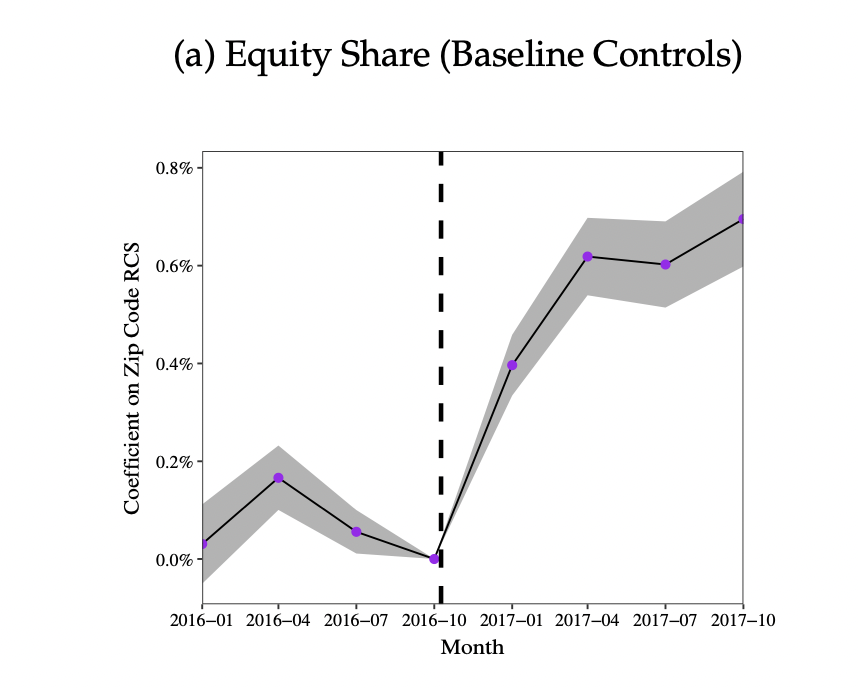
\includegraphics[width=\textwidth]{./figures/parker.png}}
	\begin{flushleft}
		{\footnotesize Note: reproduced from \cite{meeuwis2018belief}, this figure reports the baseline regression coefficients of equity share on zip-code level  campaign contribution share to Republican candidate for the three quarters prior to the election and the four quarters following the election, relative to allocations just before the election.}
	\end{flushleft}
\end{figure}


\begin{figure}[!ht] \centering  % [h!]
	\caption{A SIR model of stock investors}
		\label{fig:sir_diagram}
		\centerline{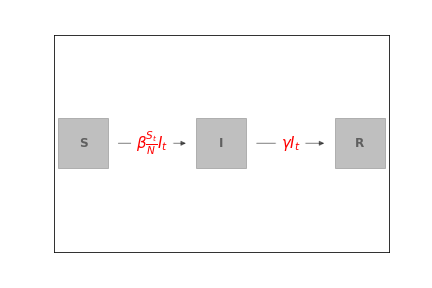
\includegraphics[width=\textwidth]{./figures/flow_diagram.png}}
		\begin{flushleft}
		{\footnotesize Note: this graph plots the transitions between different compartments in the SIR model of the stock investors as described in \cite{shiller1989survey}. }
			\end{flushleft}
	\end{figure}


\newpage

\begin{figure}[!ht] \centering  % [h!]
	\caption{Simulated trends from a SIR model of stock investors}
	\label{fig:sir_simulate}
	\centerline{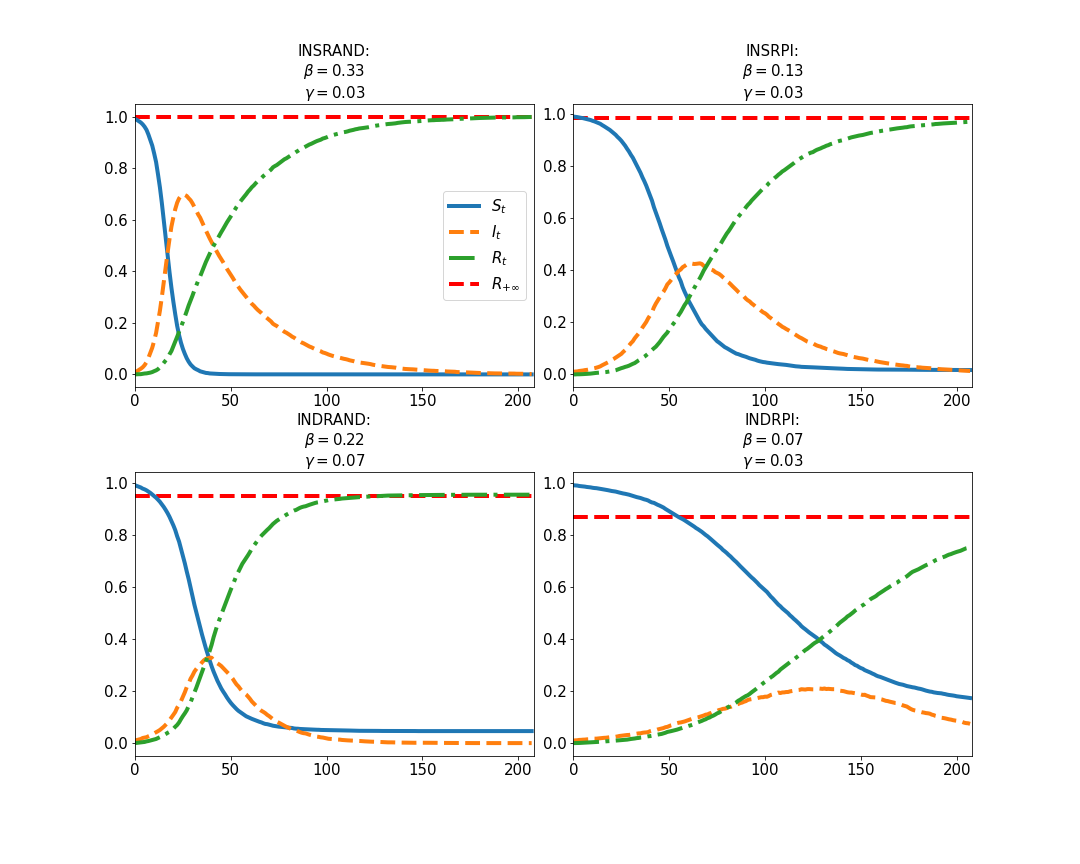
\includegraphics[width=\textwidth]{./figures/sir_simulate.png}}
	\begin{flushleft}
	{\footnotesize Note: this graph plots the simulated paths of populations in different compartments in a SIR model of stock investors, as described in \cite{shiller1989survey}. We use the median estimates of the infection rate $\beta$ and recovery rate $\gamma$ for four samples: institutional investors for a randomly selected stock (INSRAND), institutional investors for a rapidly rising stock (INSRPI), individual investors for a random stock (INDRAND), and individual investors for a rapidly rising stock (INDRPI). The horizontal dashed line corresponds to the limiting size of compartment of $R$ in the long run. The simulation is done with the Python library ``NDlib'', for details, see the companion \href{https://github.com/iworld1991/EpiExp/blob/master/Python/SIR_Ndlib.ipynb}{Jupyter Notebook}. }
				\end{flushleft}
\end{figure}




\newpage

\begin{figure}[!ht] \centering  % [h!]
	\caption{Literature map of epi models of technological diffusion}
	\label{fig:graph_diffusion}
	\centerline{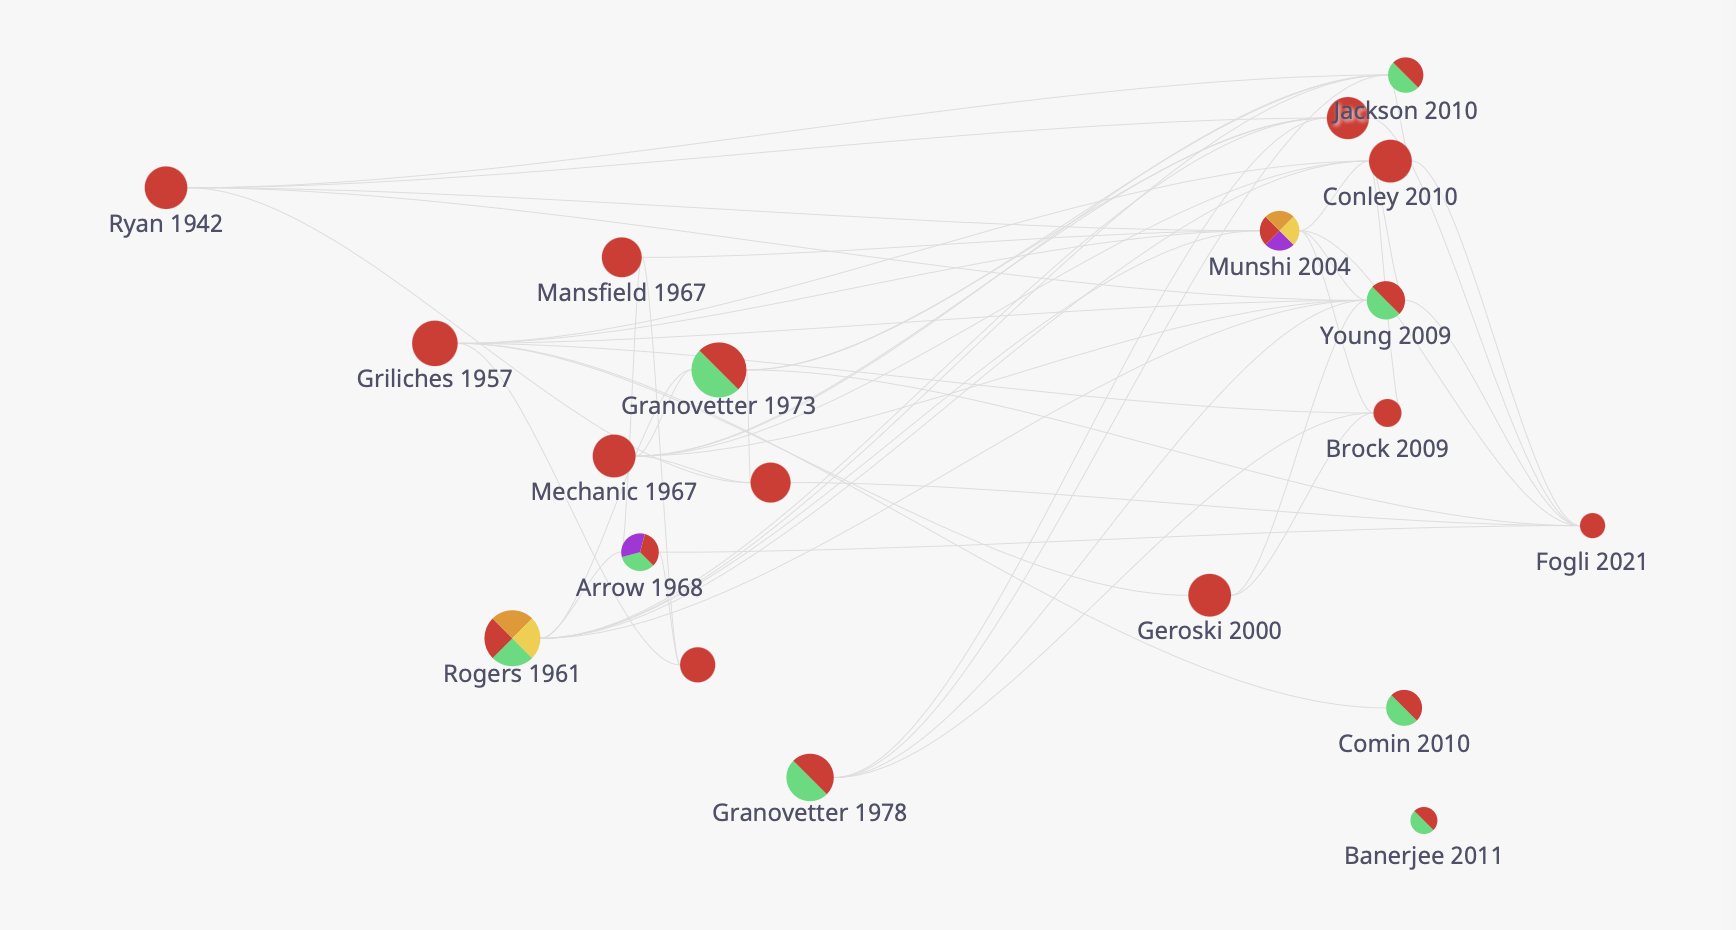
\includegraphics[width=\textwidth]{./figures/graph_diffusion.png}}
		\begin{flushleft}
{\footnotesize Note: this graph includes selected papers under the topic of epidemiological modeling of technological/innovation diffusion in economics and its related literature from other fields. See \href{https://app.litmaps.co/shared/1D9003CB-75FE-4633-B60A-79B70E03B691}{here} for its interactive version.}
				\end{flushleft}
\end{figure}


\newpage


\begin{figure}[!ht] \centering  % [h!]
	\caption{Literature on epi models of stock/housing market investment}
	\label{fig:graph_investment}
	\centerline{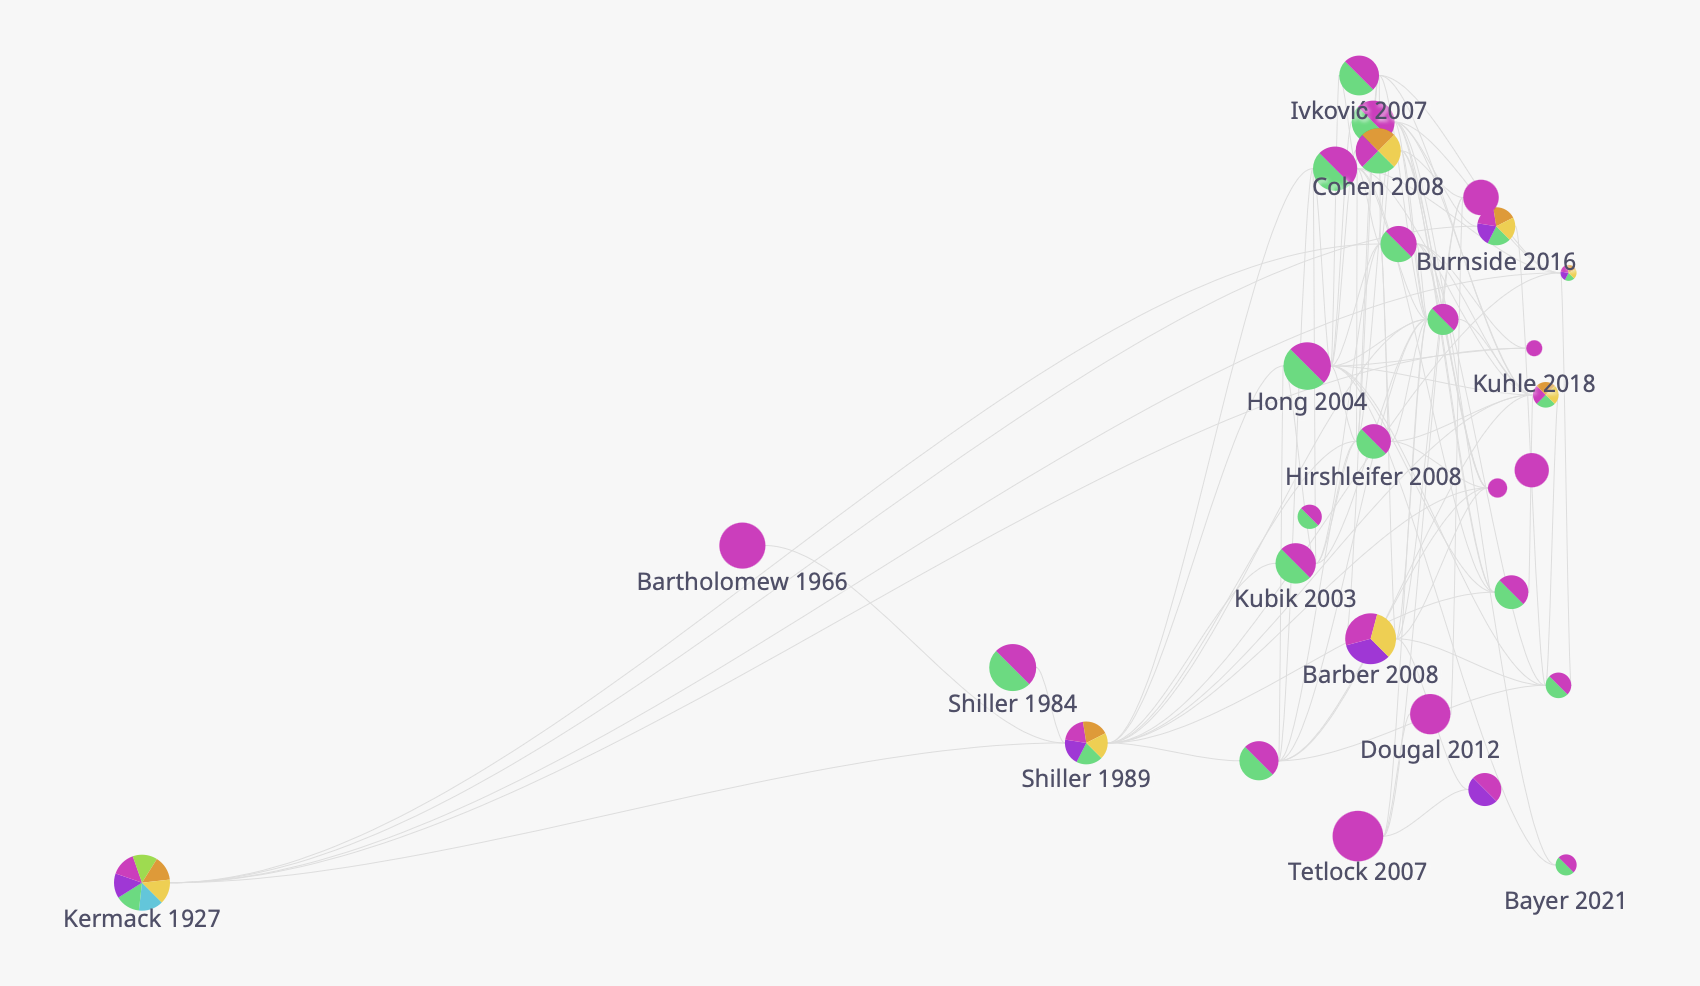
\includegraphics[width=\textwidth]{./figures/graph_investment.png}}
			\begin{flushleft}
	{\footnotesize Note: this graph includes selected papers related to epidemiological models of expectations in financial markets such as stocks and housing, and studies on the role of news media in financial markets. See \href{https://app.litmaps.co/shared/E25276CA-8725-437B-8241-11961EFB3FB4}{here} for its interactive version.}
					\end{flushleft}
\end{figure}

\newpage

\begin{figure}[!ht] \centering  % [h!]
    \hypertarget{graphmacro}{}
		\caption{Literature on epi models of macroeconomic expectations}
	\label{fig:graphmacro}
	\centerline{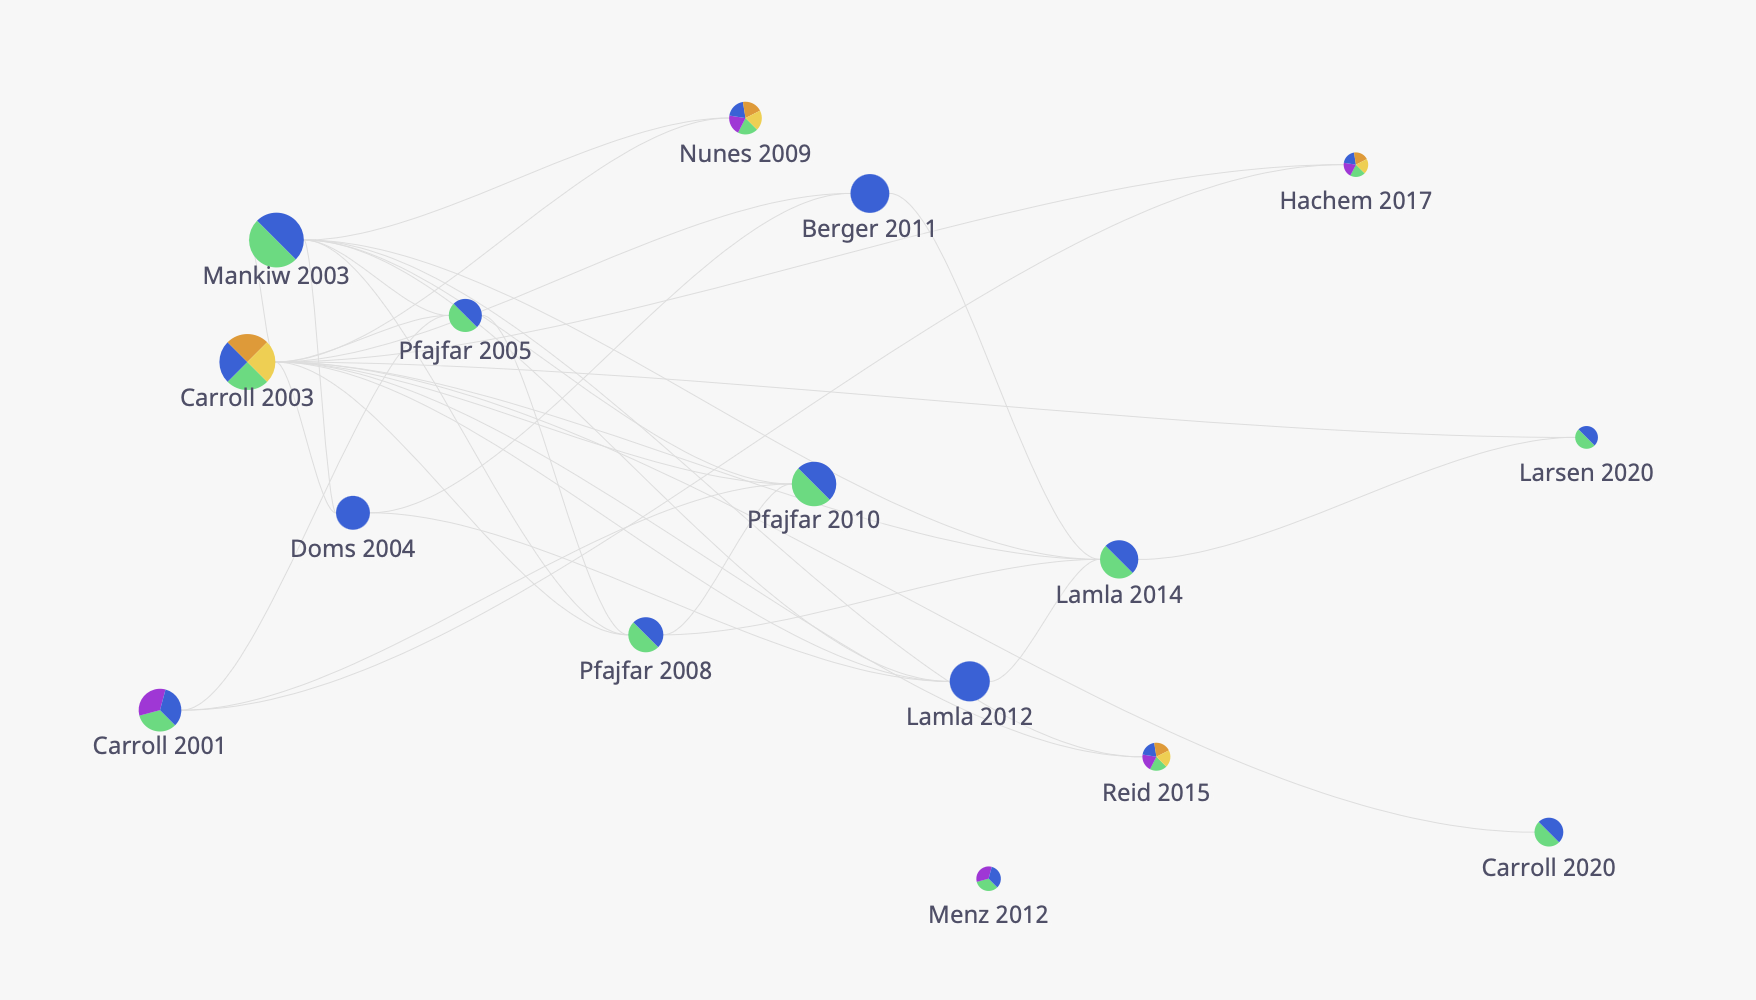
\includegraphics[width=\textwidth]{./figures/graph_macro.png}}
				\begin{flushleft}
		{\footnotesize Note: this graph includes selected papers related to epidemiological models of macroeconomic expectations, and research on the interaction between news media and macroeconomic expectations. See \href{https://app.litmaps.co/shared/289F57F4-FDE5-4F94-B1A9-2BA7419DB719}{here} for its interactive version.}
							\end{flushleft}
\end{figure}


\newpage

\begin{figure}[!ht] \centering  % [h!]
	\caption{Other fields related to epi models}
	\label{fig:graph_other}
	\centerline{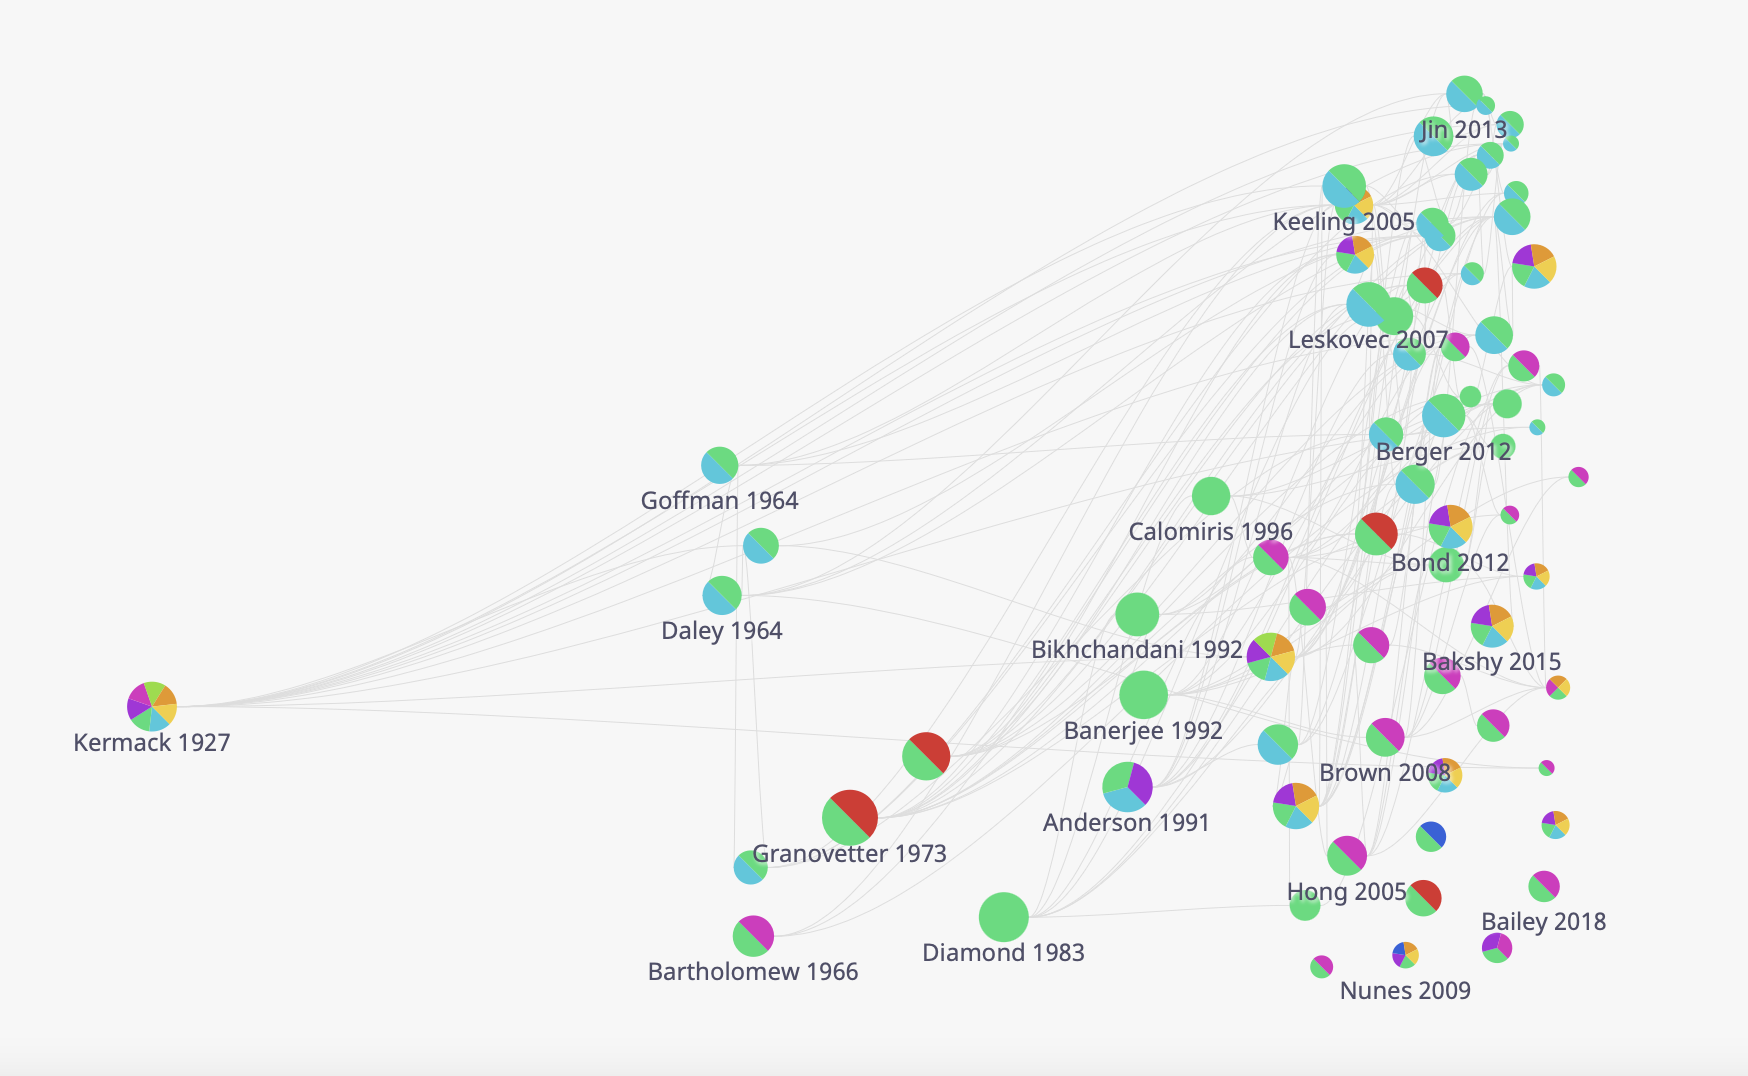
\includegraphics[width=\textwidth]{./figures/graph_other.png}}
	{\footnotesize Note: this graph includes all other papers surveyed in this chapter. It includes epi models of rumor/news/online content/scientific ideas as well as other economic research on bank runs, herd behaviors, contagion, and peer effects. See \href{https://app.litmaps.co/shared/B5FA1F14-01A8-4C9D-BF23-BE0F62293FAF}{here} for its interactive version.}
\end{figure}



\newpage


\begin{figure}[!ht] \centering  % [h!]
	\caption{\href{https://people.cs.vt.edu/ramakris/papers/news-rumor-epi-snakdd13.pdf}{\cite{jin2013epidemiological}}}
	\label{fig:news_curve}
	\centerline{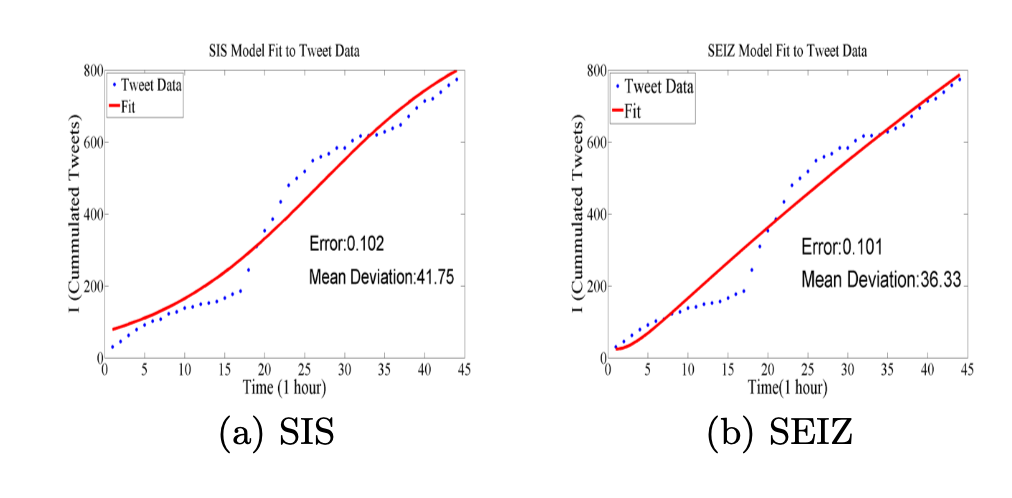
\includegraphics[width=\textwidth]{./figures/Obama.png}}

\end{figure}


\newpage
\begin{figure}[!ht] \centering  % [h!]
	\caption{\href{http://web.mit.edu/dikaiser/www/BAKC.PhysA.pdf}{\cite{bettencourt2006power}}}
	\label{fig:science_ideas_curve}
	\centerline{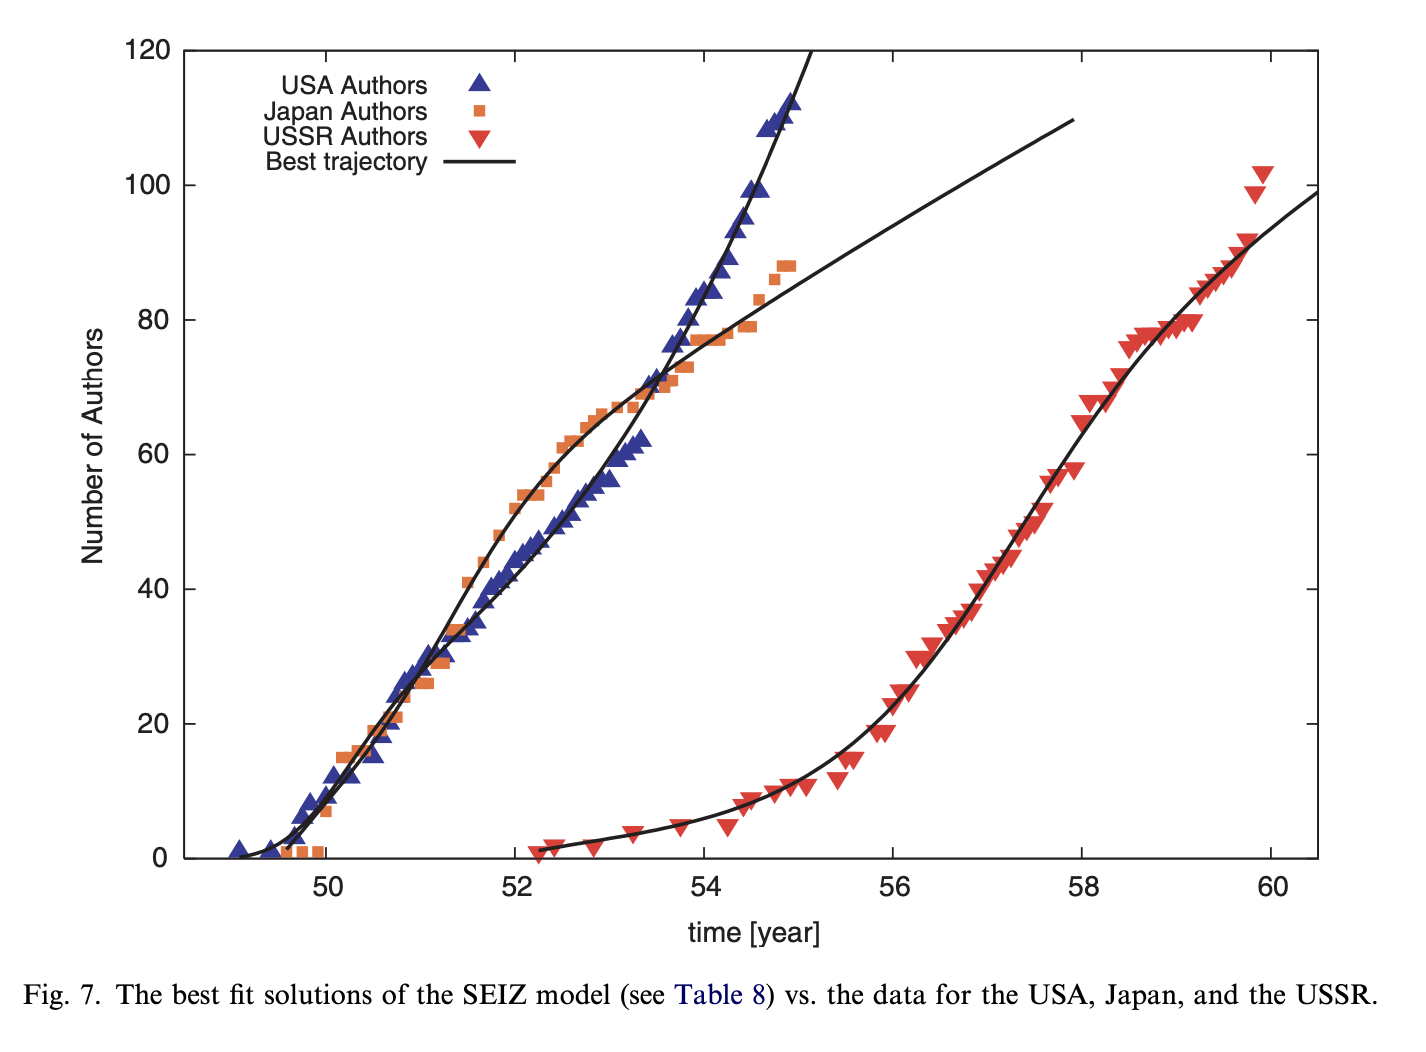
\includegraphics[width=\textwidth]{./figures/Feynman.png}}

\end{figure}


\newpage
\begin{figure}[!ht] \centering  % [h!]
	\caption{\href{https://github.com/iworld1991/EpiExp/blob/master/Literature/bauckhage2011insights.pdf}{\cite{bauckhage2011insights}}}
	\label{fig:memes_curve}
	\centerline{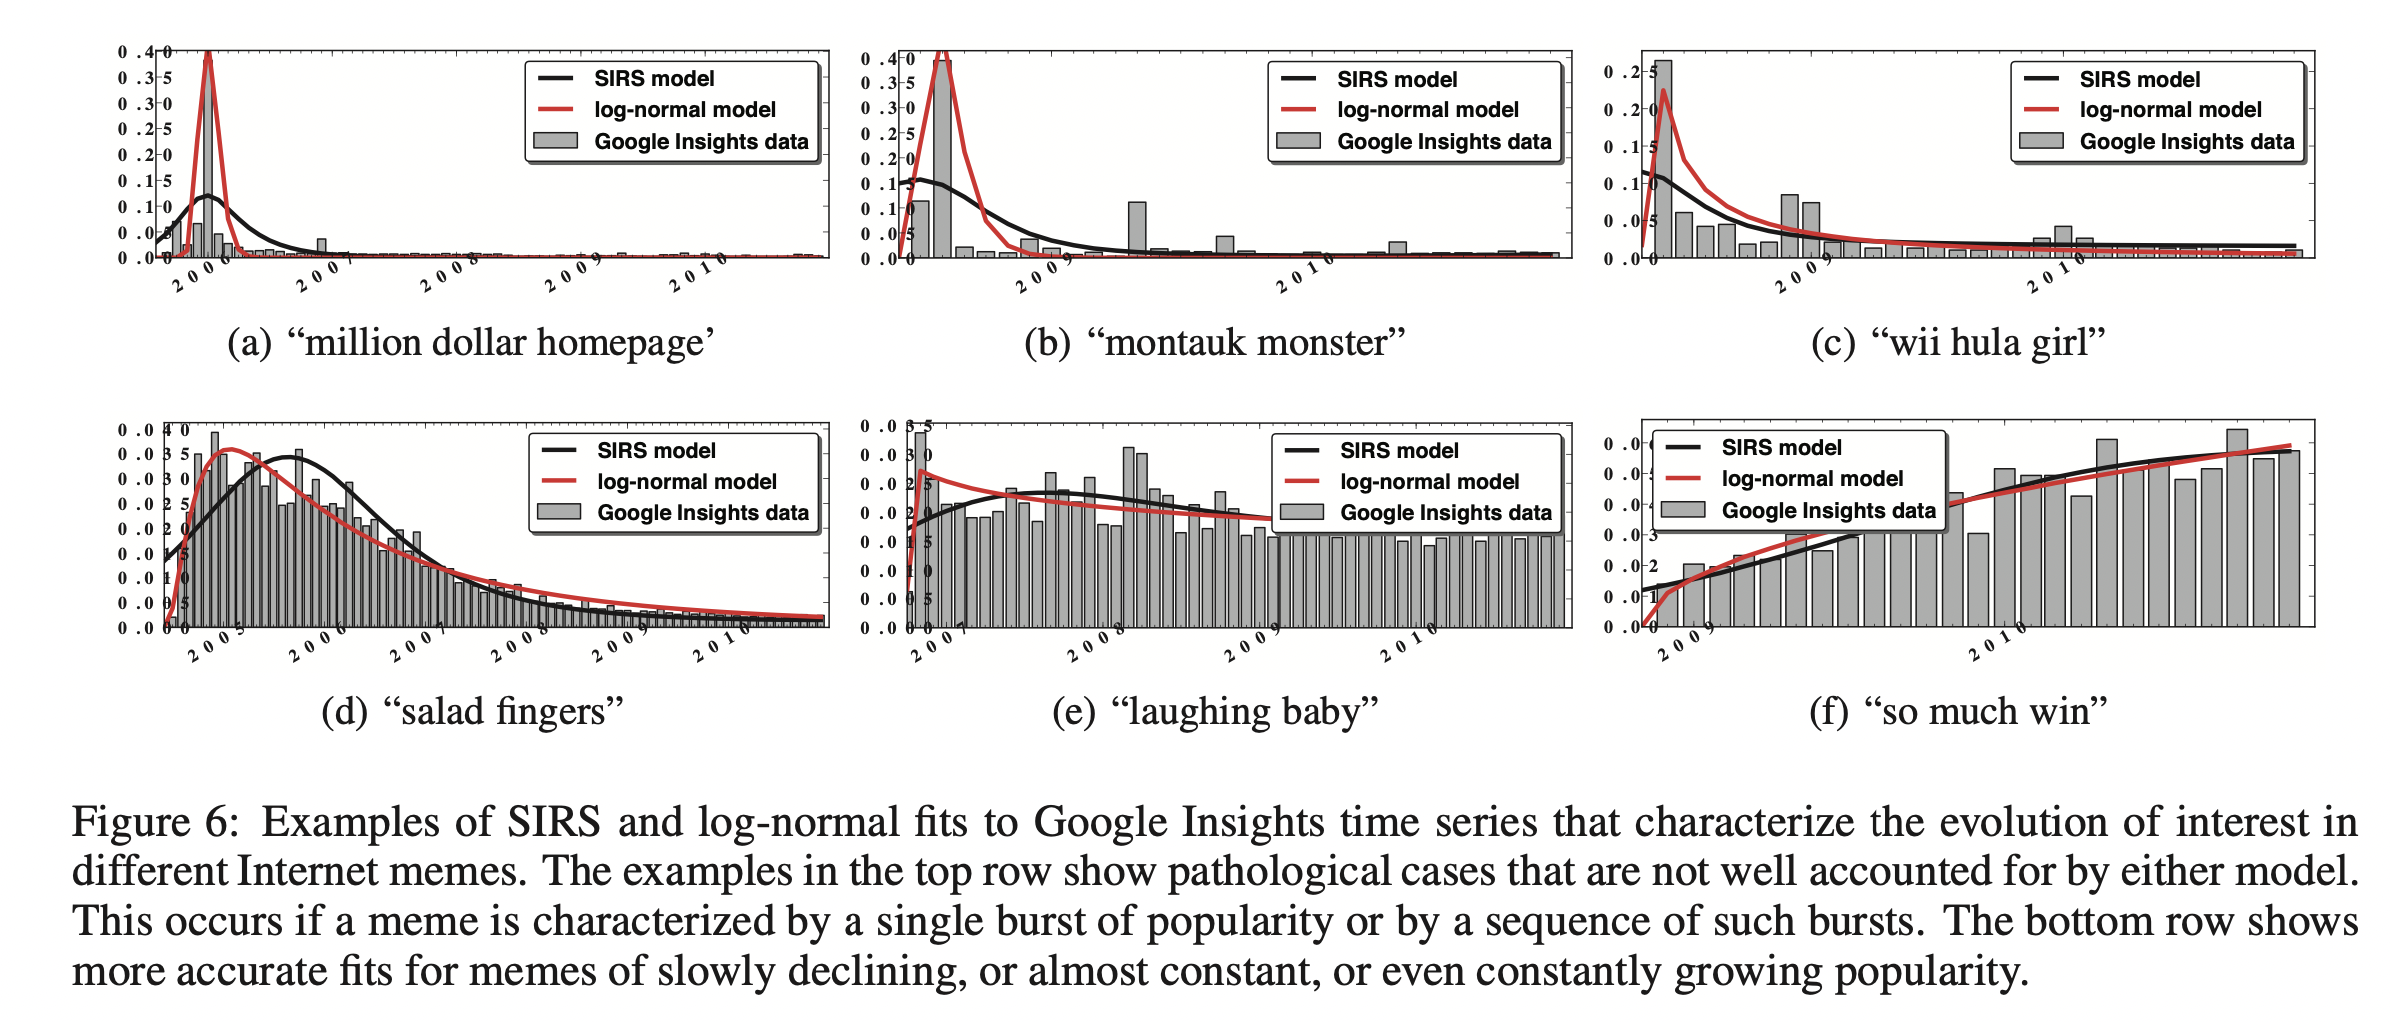
\includegraphics[width=\textwidth]{./figures/Memes.png}}

\end{figure}


\section*{REFERENCE}
\addcontentsline{toc}{section}{Reference}
\bibliographystyle{apalike}
%\bibliographystyle{plainnat}
% \bibliographystyle{Vancouver-Numbered-Style(3)}

\bibliography{reference,Add}

%
